%%%%%%%%%%%%%%%%%%%%%%%%%
% Dokumentinformationen %
%%%%%%%%%%%%%%%%%%%%%%%%%
\newcommand{\titleinfo}{Geotechnik Zusammenfassung FS18}
\newcommand{\authorname}{\href{mailto:noelle.egger@hsr.ch}{No\"elle Egger}}
\newcommand{\authoremail}{\href{mailto:noelle.egger@hsr.ch}{noelle.egger@hsr.ch}}
\newcommand{\versioninfo}{$ V0.1 $}

%%%%%%%%%%%%%%%%%%%%%%%%%%%%%%%%%%%%%%%%%%%%%
% Standard projektübergreifender Header für 
% - Makros 
% - Farben
% - Mathematische Operatoren
%
% dORT NUR ERGÄNZEN, NICHTS LÖSCHEN
%%%%%%%%%%%%%%%%%%%%%%%%%%%%%%%%%%%%%%%%%%%%%
%BuG-Fix
%Package pdf Error: Driver file ................ not found
%If you have a luatex driver fail uncomment these lines
\RequirePackage{luatex85}
\def\pgfsysdriver{pgfsys-pdftex.def}

% Genereller Header
\documentclass[10pt,twoside,a4paper,fleqn]{article}
% Dateiencoding
\usepackage[utf8]{inputenc}
\usepackage[T1]{fontenc}	%ä,ü...
% Seitenränder
\usepackage[left=1cm,right=1cm,top=0.5cm,bottom=0.5cm,includeheadfoot]{geometry}
% Sprachpaket 
\usepackage[english, ngerman]{babel} % Silbentrennung und Rechtschreibung Englisch und Deutsch

%%%%%%%%%%%%%%%%%%%%%%%
%% Wichtige Packages %%
%%%%%%%%%%%%%%%%%%%%%%%
\usepackage{amsmath}                % Allgemeine Matheumgebungen									
\usepackage{amssymb}                % Fonts: msam,msbm, eufm & Mathesymbole, Mengen (lädt automatisch amsfonts)									
\usepackage{array}                  % \newcolumntype, \firsthline, ,\lasthline, m{width}, b{width}									
\usepackage{caption}                % Bildunterschriften									
\usepackage{enumitem}               % basic environments: enumerate, itemize, description									
\usepackage{fancybox}               % \fbox: \shad­ow­box, \dou­ble­box, \oval­box, \Oval­box									
\usepackage{fancyhdr}               % Seiten schöner gestalten, insbesondere Kopf- und Fußzeile									
\usepackage{floatflt}               % Textumflossene Abbildungen \begin{floatingfigure}[r]{Breite} : r rechts, l links, p links auf geraden Seiten und rechts auf ungeraden Seiten								
\usepackage{graphicx}               % \includegraphics[keyvals]{imagefile}, [draft]graphicx zeigt nur Namen und Rahmen an, [final] hebt diese option auf => Bild wird angezeigt    									
\usepackage{hyperref}               % Erstellt Verweise innerhalb und nach außerhalb eines PDF Dokumentes.									
\usepackage{lastpage}               % Bspw. : Page 1 of 3 => \thepage\ of \pageref{LastPage}									
\usepackage{listings}               % Erlaubt es Programmcode in der gewünschten Sprache zu hinterlegen (C++, Matlab,..). Definition der Sprache mit \lstset{language=name}..									
\usepackage{longtable}              % Longtable erlaubt es Tabellen zu erstellen die bei der nächsten Seite weiterlaufen. (Bricht automatisch um)									
\usepackage{mathabx}                % Mathesymbole									
\usepackage{mathrsfs}               % \mathscr (Benötigt für Fourierreihen-Symbol)									
%\usepackage{mathtools}              % Extension package to amsmath									
\usepackage{multicol}               % multicols-Umgebung \begin{multicols}{3} erzeugt Abschnitt mit 3 Spalten									
\usepackage{multirow}               % Tabelle: ermöglicht es Felder mehrerer Zeilen in einem zusammenzufassen									
\usepackage{pdflscape}              % adds PDF support to the environment 'landscape'									
\usepackage{pxfonts}                % Symbole, griechisches Alphabet, Integrale...									
\usepackage{rotating}               % sideways, turn{degree}, rotate{degree}, sidewaysfigure, sidewaystable Umgebung									
\usepackage{subcaption}             % Bildunterschriften für Subfigures									
\usepackage{tabularx}               % tabularx-Umgebung: Hat feste Gesamtbreite, \begin{tabularx}{\textwidth}{c c c c c} X: Spalte mit variabler Breite, l, c, r, p{breite}, m{breite}									
\usepackage{textcomp}               % text symbols: baht, bullet, copyright, musical-note, onequarter, section, yen									
\usepackage{tikz}                   % Tikz Umgebung zur Grafikerzeugung									
\usepackage{titlesec}               % Überschriften zu Textabstände
\usepackage{trfsigns}               % Transformationszeichen \laplace, \Laplace..									
\usepackage{trsym}                  % Weitere Laplace Zeichen erlaubt auch vertikale Transformationszeichen									
\usepackage{verbatim}               % verbatim, verbatim*, comment Umgebung									
\usepackage{wrapfig}                % Textumflossene Bilder und Tabellen, \begin{wrapfigure}[Zeilen]{Position}[Ueberhang]{Breite}									
\usepackage{xcolor}                 % \pagecolor{color}, \textcolor{color}{text}, \colorbox{color}{text}, \fcolorbox{border-color}{fill-color}{text}									
\usepackage{titlesec}
% Zum Bilder einfach in Tabellen einfügen (valign=t)
\usepackage[export]{adjustbox}

%%%%%%%%%%%%%%%%%%%%
% Generelle Makros %
%%%%%%%%%%%%%%%%%%%%
\newcommand{\skript}[1]{$_{\textcolor{red}{\mbox{\small{Skript S.#1}}}}$}
\newcommand{\verweis}[2]{\small{(siehe auch \ref{#1}, #2 (S. \pageref{#1}))}}
\newcommand{\verweiskurz}[1]{(\small{siehe \ref{#1}\normalsize)}}
\newcommand{\subsubadd}[1]{\textcolor{black}{\mbox{#1}}}
\newcommand{\formelbuch}[1]{$_{\textcolor{red}{\mbox{\small{S#1}}}}$}

\newcommand{\kuchling}[1]{$_{\textcolor{red}{\mbox{\small{Kuchling #1}}}}$}
\newcommand{\stoecker}[1]{$_{\textcolor{grey}{\mbox{\small{Stöcker #1}}}}$}
\newcommand{\sachs}[1]{$_{\textcolor{blue}{\mbox{\small{Sachs S. #1}}}}$}
\newcommand{\hartl}[1]{$_{\textcolor{green}{\mbox{\small{Hartl S. #1}}}}$}

\newcommand{\schaum}[1]{\tiny Schaum S. #1}

\newcommand{\skriptsection}[2]{\section{#1 {\tiny Skript S. #2}}}
\newcommand{\skriptsubsection}[2]{\subsection{#1 {\tiny Skript S. #2}}}
\newcommand{\skriptsubsubsection}[2]{\subsubsection{#1 {\tiny Skript S. #2}}}

\newcommand{\matlab}[1]{\footnotesize{(Matlab: \texttt{#1})}\normalsize{}}

% Syntax: \bmu{Pfad zum Bild}{Bildgrösse}{Beschriftung des Bildes}
\newcommand{\bl}[2]{
	\begin{figure}[h]
		\flushleft  % linksbuendig
		\includegraphics[width=#1]{#2} \\
	\end{figure}
}
\newcommand{\br}[2]{
	\begin{figure}[h]
		\flushright  % rechtsbuendig
		\includegraphics[width=#1]{#2} \\
	\end{figure}
}

\newcommand{\bild}[2]{
	\begin{figure}[h]
		\centering  % zentriert
		\includegraphics[width=#1]{#2} \\
	\end{figure}
}

\newcommand\tabbild[2][]{%
	\raisebox{0pt}[\dimexpr\totalheight+\dp\strutbox\relax][\dp\strutbox]{%
		\includegraphics[#1]{#2}%
	}%
}

\newcolumntype{P}[1]{>{\raggedright\arraybackslash}p{#1}} %Tabelle linksausgerichtet
\newcolumntype{L}[1]{>{\raggedleft\arraybackslash}p{#1}} %Tabelle rechtsausgerichtet
\newcolumntype{C}[1]{>{\centering\arraybackslash}p{#1}}



%%%%%%%%%%
% Farben %
%%%%%%%%%%
\definecolor{black}{rgb}{0,0,0}
\definecolor{red}{rgb}{1,0,0}
\definecolor{white}{rgb}{1,1,1}
\definecolor{grey}{rgb}{0.8,0.8,0.8}
\definecolor{green}{rgb}{0,.8,0.05}
\definecolor{brown}{rgb}{0.603,0,0}
\definecolor{mymauve}{rgb}{0.58,0,0.82}


%%%%%%%%%%%%%%%%%%%%%%%%%%%%
% Mathematische Operatoren %
%%%%%%%%%%%%%%%%%%%%%%%%%%%%
\DeclareMathOperator{\sinc}{sinc}
\DeclareMathOperator{\sgn}{sgn}
\DeclareMathOperator{\Real}{Re}
\DeclareMathOperator{\Imag}{Im}
%\DeclareMathOperator{\e}{e}
\DeclareMathOperator{\cov}{cov}
\DeclareMathOperator{\PolyGrad}{PolyGrad}

%Grösse Integral anpassen
\def\Int{\mbox{\Large$\displaystyle\int$\normalsize}}
\def\OInt{\mbox{\Large$\displaystyle\oint$\normalsize}}

%Makro für 'd' von Integral- und Differentialgleichungen 
\newcommand*{\diff}{\mathop{}\!\mathrm{d}}

%%%%%%%%%%%%%%%%%%%%%%%%%%%
% Fouriertransformationen %
%%%%%%%%%%%%%%%%%%%%%%%%%%%

% Fouriertransformationen
\unitlength1cm
\newcommand{\FT}
{
	\begin{picture}(1,0.5)
	\put(0.2,0.1){\circle{0.14}}\put(0.27,0.1){\line(1,0){0.5}}\put(0.77,0.1){\circle*{0.14}}
	\end{picture}
}


\newcommand{\IFT}
{
	\begin{picture}(1,0.5)
	\put(0.2,0.1){\circle*{0.14}}\put(0.27,0.1){\line(1,0){0.45}}\put(0.77,0.1){\circle{0.14}}
	\end{picture}
}


%%%%%%%%%%%%%%%%%%%%%%%%%%%%
% Allgemeine Einstellungen %
%%%%%%%%%%%%%%%%%%%%%%%%%%%%

\setitemize{noitemsep,topsep=0pt,parsep=0pt,partopsep=0pt} %kompakte itemize
\setenumerate{noitemsep,topsep=0pt,parsep=0pt,partopsep=0pt} %kompakte enumerate

%Pdf Info
\hypersetup{pdfauthor={\authorname},pdftitle={\titleinfo},colorlinks=false}
\author{\authorname}
\title{\titleinfo}

% Abstände Text zu Übertiteln / Einzug
\titlespacing{\section}{12pt}{1em}{0.5em}
\titlespacing{\subsection}{12pt}{1em}{0.5em}
\titlespacing{\subsubsection}{12pt}{1em}{0.5em}

%%%%%%%%%%%%%%%%%%%%%%%
% Kopf- und Fusszeile %
%%%%%%%%%%%%%%%%%%%%%%%
\pagestyle{fancy}
\fancyhf{}
%Linien oben und unten
\renewcommand{\headrulewidth}{0.5pt} 
\renewcommand{\footrulewidth}{0.5pt}

%Kopfzeile links bzw innen
\fancyhead[L]{\titleinfo{ }\tiny{(\versioninfo)}}
%Kopfzeile mitte
%\fancyhead[C]{}
%Kopfzeile rechts bzw. aussen
\fancyhead[R]{Seite \thepage { }von \pageref{LastPage}}

%Fusszeile links bzw. innen
\fancyfoot[L]{\footnotesize{\authorname}}
%Fusszeile mitte
%\fancyfoot[C]{\footnotesize{\authoremail}}
%Fusszeile rechts bzw. ausen
\fancyfoot[R]{\footnotesize{\today}}
% Einrücken verhindern versuchen
\setlength{\parindent}{0pt}

%%%%%%%%%%%%%%%%%%%%%%%%%%%%%%%%%%%%%%%
%% Makros & anderer Low-Level bastel %%
%%%%%%%%%%%%%%%%%%%%%%%%%%%%%%%%%%%%%%%
% Zeilenhöhe Tabellen:
\newcommand{\arraystretchOriginal}{1.5}
\renewcommand{\arraystretch}{\arraystretchOriginal}

\makeatletter
%% Makros für den Arraystretch (bei uns meist in Tabellen genutzt, welche Formeln enthalten)
% Default Value
\def\@ArrayStretchDefault{1} % Entspricht der Voreinstellung von Latex

% Setzt einen neuen Wert für den arraystretch
\newcommand{\setArrayStretch}[1]{\renewcommand{\arraystretch}{#1}}

% Setzt den arraystretch zurück auf den default wert
\newcommand{\resetArrayStretch}{\renewcommand{\arraystretch}{\@ArrayStretchDefault}}

% Makro zum setzten des Default arraystretch. Kann nur in der Präambel verwendet werden.
\newcommand{\setDefaultArrayStretch}[1]{%
    \AtBeginDocument{%
        \def\@ArrayStretchDefault{#1}
        \renewcommand{\arraystretch}{#1}
    }
}
\makeatother

%% Achtung Symbol \danger
\newcommand*{\TakeFourierOrnament}[1]{{%
        \fontencoding{U}\fontfamily{futs}\selectfont\char#1}}
\newcommand*{\danger}{\TakeFourierOrnament{66}}


%%%%%%%%%%%%%%%%
% Code Layout %
%https://en.wikibooks.org/wiki/LaTeX/Source_Code_Listings
%%%%%%%%%%%%%%%

\definecolor{mygreen}{rgb}{0,0.6,0}
\definecolor{mygray}{rgb}{0.5,0.5,0.5}
\definecolor{mymauve}{rgb}{0.58,0,0.82}

\lstset{ %
    firstnumber=1,
    backgroundcolor=\color{white},   % choose the background color; you must add        \usepackage{color} or \usepackage{xcolor}
    basicstyle=\footnotesize\ttfamily, % the size of the fonts that are used for the code
    breakatwhitespace=false,         % sets if automatic breaks should only happen at whitespace
    breaklines=true,                 % sets automatic line breaking
    captionpos=b,                    % sets the caption-position to bottom
    commentstyle=\color{mygreen},    % comment style
    deletekeywords={...},            % if you want to delete keywords from the given language
    otherkeywords={...},             % if you want to add more keywords to the set
    escapeinside={\%*}{*\%},          % if you want to add LaTeX within your code
    extendedchars=true,              % lets you use non-ASCII characters; for 8-bits encodings only, does not work with UTF-8
    frame=single,	                 % adds a frame around the code
    keepspaces=true,                 % keeps spaces in text, useful for keeping indentation of code (possibly needs columns=flexible)
    keywordstyle=\color{blue},       % keyword style
    language=C++,                    % the language of the code   
    numbers=left,                    % where to put the line-numbers; possible values are (none, left, right)
    numbersep=5pt,                   % how far the line-numbers are from the code
    numberstyle=\tiny\color{mygray}, % the style that is used for the line-numbers
    rulecolor=\color{black},         % if not set, the frame-color may be changed on line-breaks within not-black text (e.g. comments (green here))
    showspaces=false,                % show spaces everywhere adding particular underscores; it overrides 'showstringspaces'
    showstringspaces=false,          % underline spaces within strings only
    showtabs=false,                  % show tabs within strings adding particular underscores
    stepnumber=2,                    % the step between two line-numbers. If it's 1, each line will be numbered
    stringstyle=\color{mymauve},     % string literal style
    tabsize=2,	                     % sets default tabsize to 2 spaces
    %title=\lstname                   % show the filename of files included with         \lstinputlisting; also try caption instead of title
}

\lstdefinestyle{customc++}{
    belowcaptionskip=1\baselineskip,
    %frame=L,
    xleftmargin=\parindent,
    language=C++,
    keywordstyle=\bfseries\color{blue},
    commentstyle=\itshape\color{mygreen},
    identifierstyle=\color{black},
    stringstyle=\color{gray},
}

\lstdefinestyle{cppunit}{
    belowcaptionskip=1\baselineskip,
    %frame=L,
    xleftmargin=\parindent,
    language=C++,
    keywordstyle=\bfseries\color{blue},
    keywordstyle=[2]\bf\color{black}, %not sure why \bf works, but it does
    commentstyle=\itshape\color{mygreen},
    identifierstyle=\color{black},
    stringstyle=\color{gray},
    keywords=[2]{  %Cpp Unit Keywords
        CPPUNIT_ASSERT,
        CPPUNIT_TEST,
        CPPUNIT_TEST_EXCEPTION,
        CPPUNIT_TEST_END,
        CPPUNIT_TEST_SUITE,
        CPPUNIT_TEST_SUITE_REGISTRATION,
        CPPUNIT_TEST_SUITE_END},
}

\lstdefinestyle{cppqt}{
    belowcaptionskip=1\baselineskip,
    %frame=L,
    xleftmargin=\parindent,
    language=C++,
    keywordstyle=\bfseries\color{blue},
    keywordstyle=[2]\bfseries\color{red},
    commentstyle=\itshape\color{mygreen},
    identifierstyle=\color{black},
    stringstyle=\color{gray},
    keywords=[2]{           % qt-Keywords
		Qt,
        SIGNAL,
        SLOT,
        QApplication,
        QDialog,
        QGridLayout,
        QPushButton,
        QLabel,
        QVBoxLayout,
        QHBoxLayout,
        QWidget,
        QGroupBox,
        QFont,
        QLineEdit,
        QRadioButton,
        QPen,
        QRect,
        QPaintEvent,
        QBrush,
        QPixmap,
        QPainter,
        QString,
        QPoint,
        update()},
}

\lstdefinestyle{cdoxy}{
    belowcaptionskip=1\baselineskip,
    %frame=L,
    xleftmargin=\parindent,
    language=C++,  
    keywordstyle=\bfseries\color{blue},
    commentstyle=\itshape\color{mygreen},
    identifierstyle=\color{black},
    stringstyle=\color{gray},
    otherkeywords={           % DoxygenKeywords
        ...,
        ....,
        @mainpage,
        @file,
        @author,
        @version,
        @date,
        @bug,
        @brief,
        @extended,
        @param,
        @return,
        @warning,
        @note,
        @see},
}

%choose customstyle in DOC with \lstinputlisting[style=custom]{path}
\lstset{style=customc++}

% Möglichst keine Ergänzungen hier, sondern in header.tex

%%%%%%%%%%%%%%%%%%%%%%%%%%%%%%%%%%%%%%%%%%%%%%%%%%%%%%%%%%%%%%%%%%%%%%%%%%%%%%%%%%%%%%%%%%%%%%%%
%%%%%%%%%%%%%%%%%%%%%%%%%%%%%%%%%%%%%%%%%%%%%%%%%%%%%%%%%%%%%%%%%%%%%%%%%%%%%%%%%%%%%%%%%%%%%%%%

\begin{document}
\maketitle
\tableofcontents
\thispagestyle{empty}
\newpage



	

\begin{minipage}{0.35\linewidth}
\section{Flachfundationen}
	\subsection{Tragfähigkeit}
		\textbf{Vorgehen}
		\begin{enumerate}
			\item Einwirkende Kraft E$_d$ = F$_{z,tot}$
			\item Bruchspannung $\sigma_f $
			\item vorhandene Spannung $ \sigma_v = \frac{ F_{z,tot,d} }{ \bar{a} \cdot \bar{b} } $
			\item Nachweis $ E_d \leq R_d $
		\end{enumerate}
%	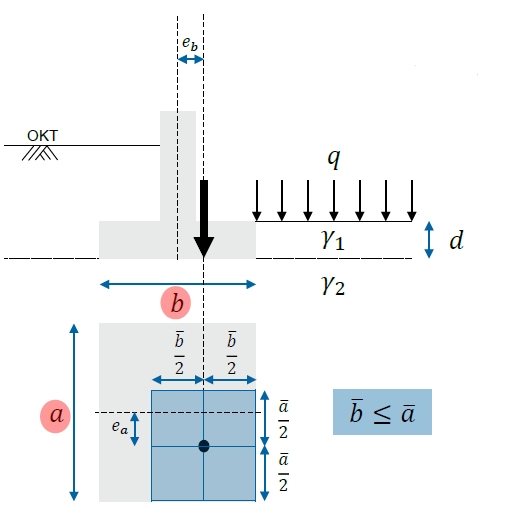
\includegraphics[width=0.7\linewidth]{images/Flachfun1allgTragfah.PNG}
\end{minipage}
\begin{minipage}{\linewidth}
	\begin{tabular}{l|p{0.2\linewidth}}
		\multicolumn{2}{c}{\textbf{Statistik} } \\ \hline
		
		Mittelwert							&	$ x_m = \frac{1}{n} \sum x_i $	\\
		
		Standardabweichung der Stichprobe	& 	$ s = \sqrt{ \frac{1}{n - 1} \sum (x_i - x_m)^2 } $ \\
		
		Charakteristischer Wert				&	$ s_{u,k} = \varphi_k' = x_m - \frac{s}{\sqrt{n} } \cdot c $
												$ \rightarrow$ c-Wert aus Tabelle; $ f = n - 1; p = 1 -\alpha$	\\ 
		
		Berechnungswert $ \varphi_d' $		&	$ \varphi_d' = arctan (\frac{tan \varphi_k'}{1.2}) $ \\ \hline
		
	\end{tabular}
\end{minipage}	
\begin{minipage}{0.8\linewidth}
	
		\begin{tabular}{|l|l|p{0.25\linewidth}|}
			\hline
			Formel			&	Einheit		&	Bemerkung \\ \hline
			
			$ R_n
			= \bar{a} \cdot \bar{b} \cdot \sigma $ & [kN] & Bruchkraft; Achtung: Formel gilt für $ d/b \leq 2 $ \\ 
			$ \bar{a}
			= a - 2 \cdot e_a $ &	[m]		& reduzierter QS-Wert	\\
			$ e_a
			= \frac{M_y}{F_z} $ &	[m]		& Exzentrizität	\\
			$ \bar{b}
			= b - 2 \cdot e_b $ &	[m]		& reduzierter QS-Wert	\\
			$ e_b
			= \frac{M_x}{F_z} $ &	[m]		& Exzentrizität	\\
			$ \sigma_{f}
			= \gamma_2 \cdot \bar{b} \cdot N_b + ( \gamma_1 \cdot d + q ) \cdot N_d + c \cdot N_c $	& $ \left[\frac{kN}{m^3}\right] $ / [kPa]	& Bruchspannung,	c = Kohäsion \\		\hline
%			$ N_b
%			= N_{b0} \cdot \nu_b \cdot \iota_b \cdot \lambda_b \cdot \xi_b $
%			& $ \left[\frac{kN}{m^3}\right] $		&	\\
%			$ N_{b0}
%			= ( N_{d0} - 1 ) \cdot tan (\varphi) $ & [kN]	& undrainiert: $ N_{b0} = 0 $\\
%			$ N_d
%			= N_{d0} \cdot \nu_d \cdot \iota_d \cdot \lambda_d \cdot \xi_d $
%							& $ \left[\frac{kN}{m^3}\right] $		&	\\
%			$ N_{d0}
%			= e^{ \pi \cdot tan ( \varphi) } \cdot tan^2 ( 45° + \frac{\varphi}{2} ) $ & [kN]	& undrainiert: $ \varphi_u = 0 $;  $ N_{d0} = 1 $ \\
%						&		& drainier: $ \varphi ' > 0 $ 	\\
%			$ \nu_d
%			= 1 + \frac{\bar{b}}{\bar{a}} \cdot \sin(\varphi) $ &			&	\\
%			$ \iota_d
%			= ( 1 - tan(\delta))^m $	&		&	\\
%			$ \delta
%			= arctan \left( \frac{T}{F_z}\right) $		 & $\degree$		& 3 dimensionaler Winkel	\\
%			$ T
%			= \sqrt{F_x^2 + F_y^2} $ & $ \left[\frac{kN}{m^3}\right] $ &	Resultierende \\	
%			$ m
%			= m_a \cdot cos^2 (\omega) + m_b \cdot sin^2 (\omega) $ & &	\\
%			$ m_a
%			= \frac{2 + \frac{\bar{a}}{\bar{b}}}{1 + \frac{\bar{a}}{\bar{b}}} $ & & \\
%			$ m_b
%			= \frac{2 + \frac{\bar{b}}{\bar{a}}}{1 + \frac{\bar{b}}{\bar{a}}} $ & & \\	
%			$ \omega
%			= arctan \left[ \frac{F_y}{F_x} \right] $ &  & \\
%			$ \lambda_d
%			= 1 - 0.4 \cdot tan ( \beta ) $ &		&	\\ 
%			$ N_c
%			= N_{c0} \cdot \nu_c \cdot \iota_c \cdot \lambda_c \cdot \xi_c $
%			& $ \left[\frac{kN}{m^3}\right] $		&	\\
%			$ N_{c0}
%			= ( N_{d0} - 1) \cdot cot (\varphi) $ & [kN]	& undrainiert: $ N_{c0} = 2 + \pi $ \\ \hline
		\end{tabular}
	
\end{minipage}
\begin{minipage}{0.25\linewidth}
	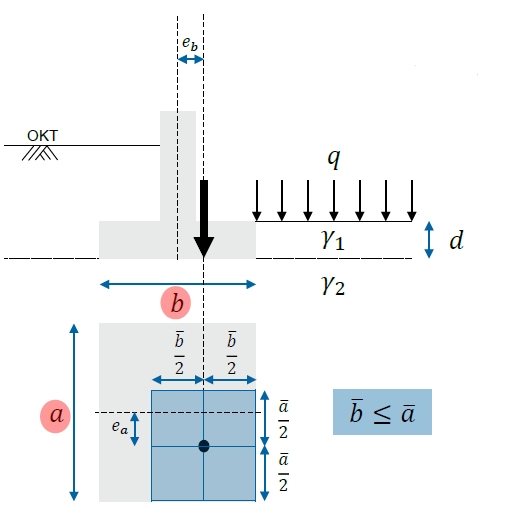
\includegraphics[width=\linewidth]{images/Flachfun1allgTragfah.PNG}
\end{minipage}


\begin{minipage}{0.85\linewidth}
	\begin{tabular}{l|l|ll}
		Bemerkung	& drainiert $ \varphi ' > 0 $	& undrainiert $ \varphi_u = 0 $ & \\ \hline
		
		Tragfähigkeitbeiwerte	& $ N_b
									= N_{b0} \cdot \nu_b \cdot \iota_b \cdot \lambda_b \cdot \xi_b $											& &	\\
								& $ N_d
								= N_{d0} \cdot \nu_d \cdot \iota_d \cdot \lambda_d \cdot \xi_d $	& & \\
								& $ N_c
								= N_{c0} \cdot \nu_c \cdot \iota_c \cdot \lambda_c \cdot \xi_c $ & & \\ \hline
								& $ N_{b0}
								= ( N_{d0} - 1 ) \cdot tan (\varphi) $	& $ N_{b0} = 0 $ & \\
								& $ N_{d0}
								= e^{ \pi \cdot tan ( \varphi) } \cdot tan^2 ( 45° + \frac{\varphi}{2} ) $ & $ N_{d0} = 1 $ & \\
								& $ N_{c0}
								= ( N_{d0} - 1) \cdot cot (\varphi) $ & $ N_{c0} = 2 + \pi $ & \\ \hline
		Formbeiwert				& $ \nu_b
								= 1 - 0.3 \cdot \frac{\bar{b}}{\bar{a}} $	& $ \nu_b = 1 $ & \\
								& $ \nu_d
								= 1 + \frac{\bar{b}}{\bar{a}} \cdot \sin(\varphi) $ & $ \nu_d = 1 $ & \\
								& $ \nu_c = \frac{\nu_d \cdot N_{d0} -1}{N_{d0} -1} $ & $ \nu_c = 1 + 0.2 \cdot \frac{\bar{b}}{\bar{a}} $ & \\ \hline
		Lastneigungsbeiwert $ \delta > 0 $		& $ \iota_b = (1 - tan ( \delta [\degree] ) ) ^{(m+1)} $	& & \\
								& $ \iota_d = (1 - tan ( \delta [\degree] ) ) ^m $	& $ \iota_d = 1 $  & \\
								& $ \iota_c = \frac{\iota_d \cdot N_{d0} -1}{N_{d0} -1} $ & $ \iota_c = \frac{1}{2} + \frac{1}{2} \cdot \sqrt{1 - \frac{T}{\bar{a} \cdot \bar{b} \cdot c_u}} $ & 					% 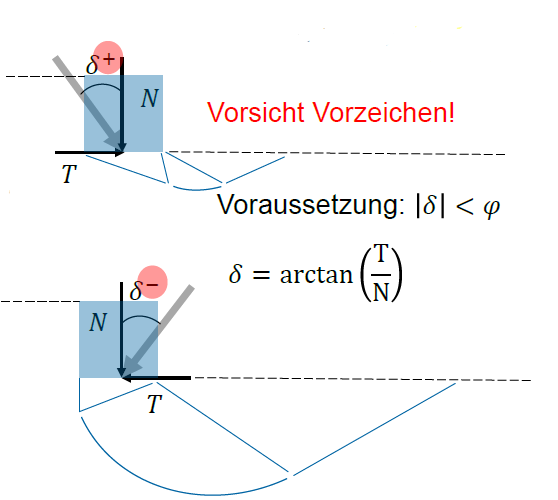
\includegraphics[width=0.2\linewidth]{images/Flachfun2Vorz.PNG} 
								\\
		Lastneigungsbeiwert $ \delta > 0 $ 	& $ \iota_b = cos ( \delta [\degree] ) \cdot (1 - 0.4 \cdot \delta [\degree]) ^{(0.64 + 0.028 \cdot \varphi [\degree])} $ & & \\
								& $ \iota_d = cos (\delta [\degree]) \cdot (1 - 0.0244 \cdot \delta [\degree]) ^{(0.03 + 0.04 \cdot \varphi [\degree])} $ & & \\
								& $ \iota_c = \frac{\iota_d \cdot N_{d0} -1}{N_{d0} -1} $ & & \\
								&&& \\
		3 dimensionaler Winkel	& $ \delta = arctan \left( \frac{T}{F_z}\right) $		 & 	& 	\\
		Resultierende			& $ T = \sqrt{F_x^2 + F_y^2} $ &  &	 \\
								& $ m = m_a \cdot cos^2 (\omega) + m_b \cdot sin^2 (\omega) $ & & \\
								& $ \omega = arctan \left[ \frac{F_y}{F_x} \right] $ &  & \\
								& $ m_a = \frac{2 + \frac{\bar{a}}{\bar{b}}}{1 + \frac{\bar{a}}{\bar{b}}} $ & & \\
								& $ m_b = \frac{2 + \frac{\bar{b}}{\bar{a}}}{1 + \frac{\bar{b}}{\bar{a}}} $ & & % 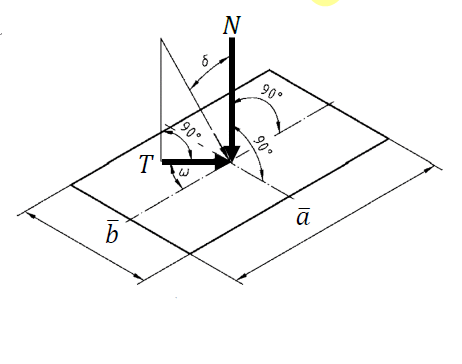
\includegraphics[width=0.2\linewidth]{images/Flachfun2Winkel.PNG} 
								\\ \hline
		Geländeneigungsbeiwert & $ \lambda_b = (1 - \frac{1}{2} \cdot tan (\beta [\degree] ) ) ^6 $ 	& & \\
								& $ \lambda_d = (1 - tan (\beta [\degree] ) ) ^{1.9} $	& $ \lambda_d = 1 $ & \\
								& $ \lambda_c = \frac{N_{d0} \cdot e ^{ (-0.0349 \cdot \beta [°] \cdot tan (\varphi [\degree] ) ) } -1 }{N_{d0} - 1} $	& $ \lambda_c = 1- 0.4 \cdot tan ( \beta [\degree] ) $ \\
								&	& $ \rightarrow $wenn $ \beta < \varphi $ & %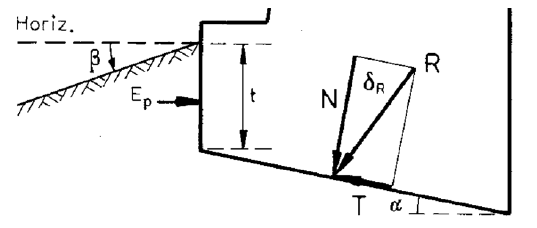
\includegraphics[width=0.2\linewidth]{images/Flachfun3Neig.PNG}
								\\ \hline 
		Sohlneigungsbeiwert		& $ \xi_b = e ^{(-0.045 \cdot \alpha [\degree] \cdot tan (\varphi [\degree]))} $	&	& \\
								& $ \xi_d = e ^{(-0.045 \cdot \alpha [\degree] \cdot tan (\varphi [\degree]))} $	& $ \xi_d = 1 $ & \\
								& $ \xi_c = e ^{(-0.045 \cdot \alpha [\degree] \cdot tan (\varphi [\degree]))} $ & $ \xi_c = 1 - 0.0068 \cdot \alpha [\degree] $ & %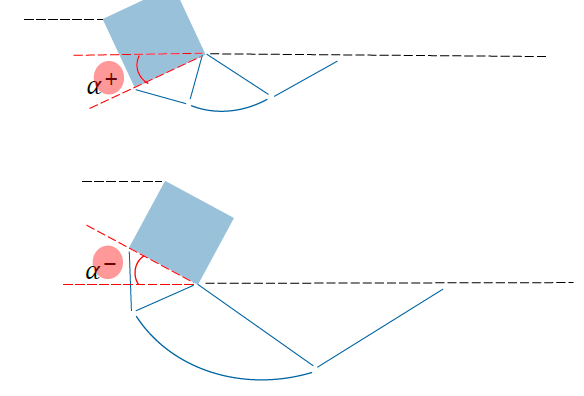
\includegraphics[width=0.2\linewidth]{images/Flachfun4Winkel.PNG} 
								\\ \hline			
		
	\end{tabular}
\end{minipage}
\begin{minipage}{0.2\linewidth}
	
	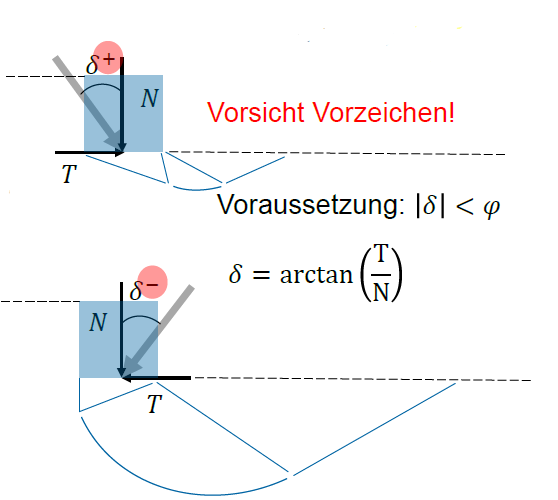
\includegraphics[width=\linewidth]{images/Flachfun2Vorz.PNG} \\
	
	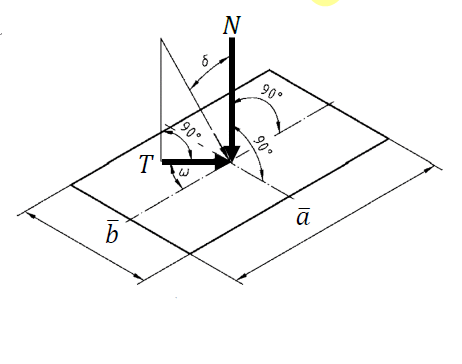
\includegraphics[width=\linewidth]{images/Flachfun2Winkel.PNG} \\
	
	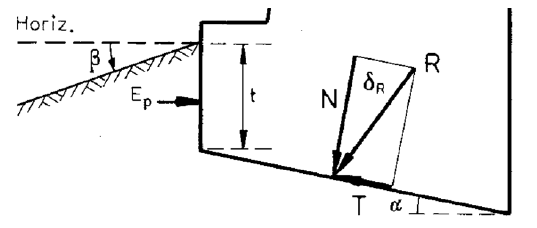
\includegraphics[width=\linewidth]{images/Flachfun3Neig.PNG} \\
	
	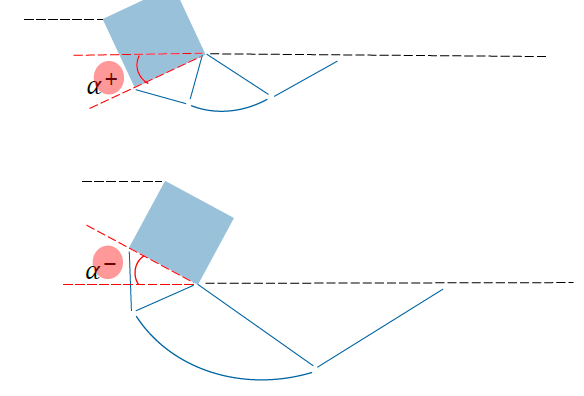
\includegraphics[width=\linewidth]{images/Flachfun4Winkel.PNG} \\
	
\end{minipage}


\textcolor{red}{Sicherheitsbeiwerte Geotech}



%	\subsection{Statistik}
	
%	\begin{minipage}{\linewidth}
%		\begin{tabular}{l|p{0.3\linewidth}}
%			 \hline
%			Mittelwert							&	$ x_m = \frac{1}{n} \sum x_i $	\\
%			
%			Standardabweichung der Stichprobe	& 	$ s = \sqrt{ \frac{1}{n - 1} \sum (x_i - x_m)^2 } $ \\
%				
%			Charakteristischer Wert				&	$ f = n - 1; p = 1 -\alpha$; c-Wert aus Tabelle $ \rightarrow s_{u,k} = \varphi_k' = x_m - \frac{s}{\sqrt{n} } \cdot c $	\\ 
%			
%			Berechnungswert $ \varphi_d' $		&	$ \varphi_d' = arctan (\frac{tan \varphi_k'}{1.2}) $ \\ \hline
%						
%		\end{tabular}
%	\end{minipage}	



	\begin{minipage}{0.5\linewidth}
		\subsection{Gebrauchstauglichkeit}
			\subsubsection{Relative Steifigkeit}
			$ k = \frac{1}{12} \frac{E}{M_E} \left( \frac{d}{l} \right)^3 $ \\
		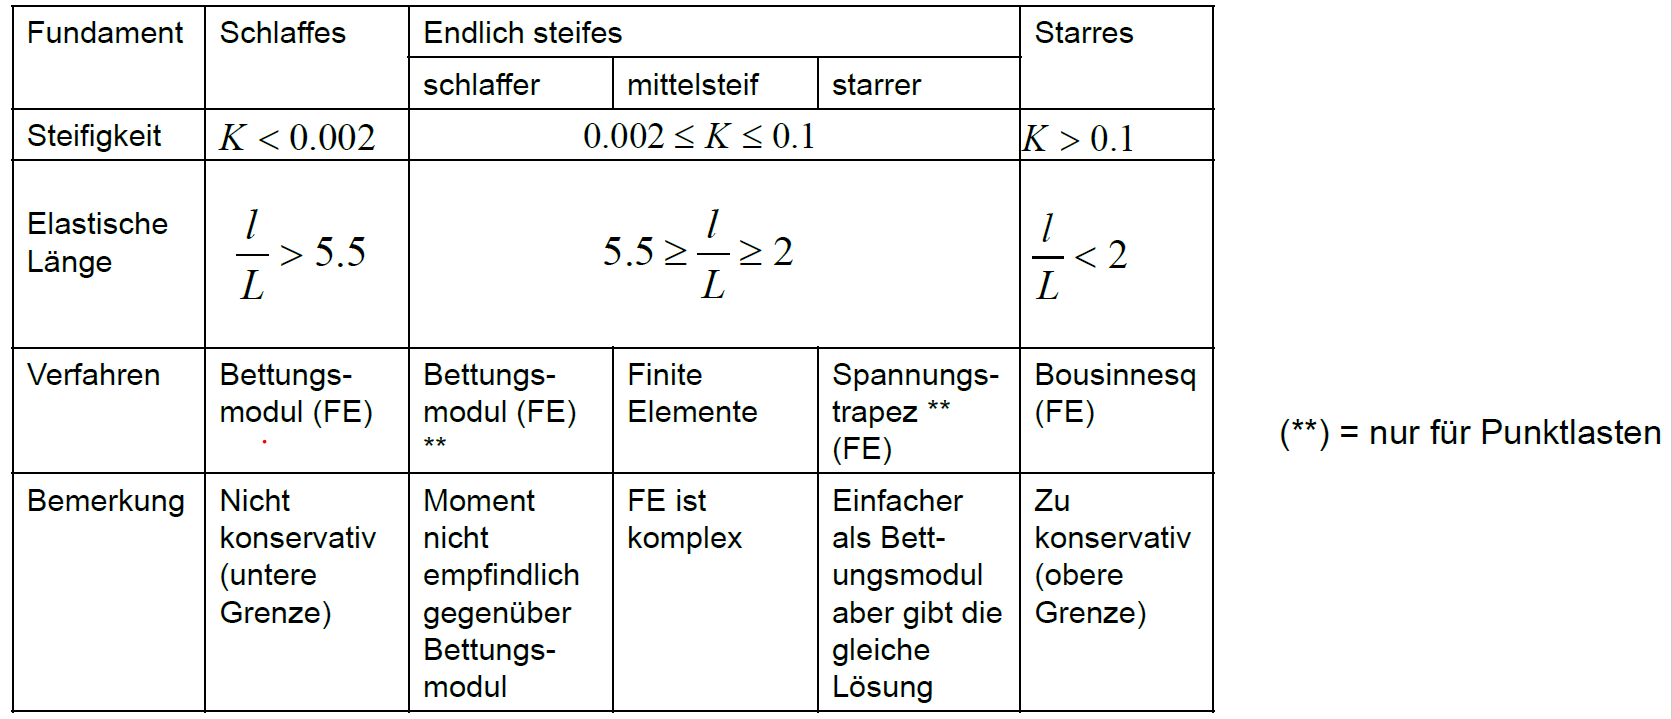
\includegraphics[width=\linewidth]{images/Flachfun5starrschlaff.PNG}
	\end{minipage}
	\begin{minipage}{0.3\linewidth}
		\subsubsection{Spannungstrapezverfahren}
		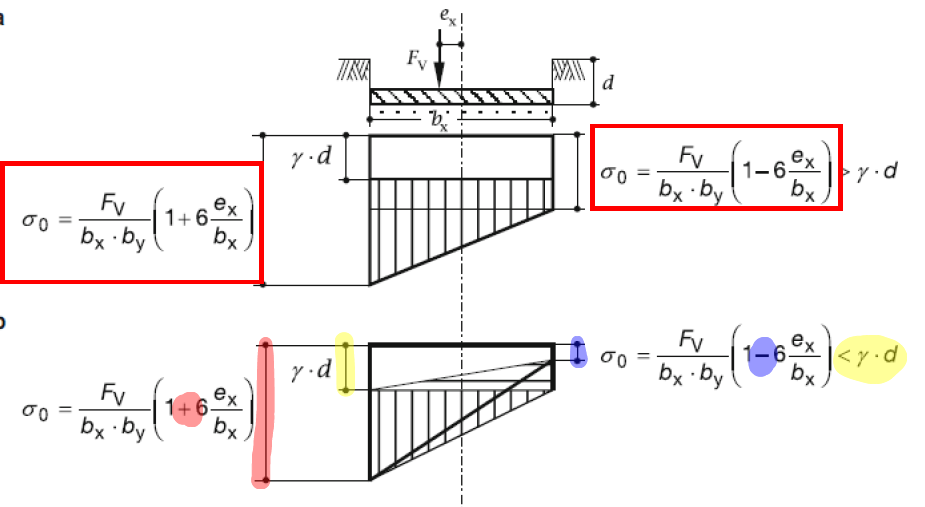
\includegraphics[width=\linewidth]{images/Flachfun6Sptrapez.PNG}
	\end{minipage}



%\begin{minipage}{\linewidth}
%	\begin{tabular}{l|l|l}
%		Formel			&	Einheit	&	Bemerkung \\ \hline
%	\end{tabular}
%\end{minipage}
\clearpage


\begin{minipage}{0.35\linewidth}

\section{Grundwasser}

	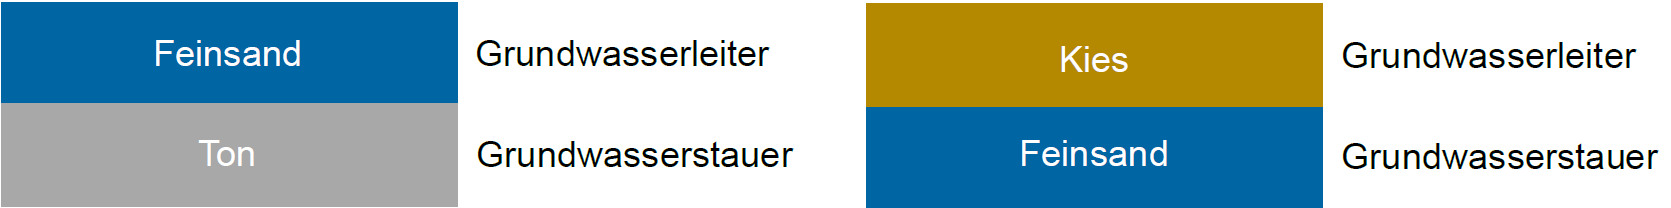
\includegraphics[width=\linewidth]{images/GW1Stauer.PNG} \\
%\end{minipage}
%\begin{minipage}{0.5\linewidth}
	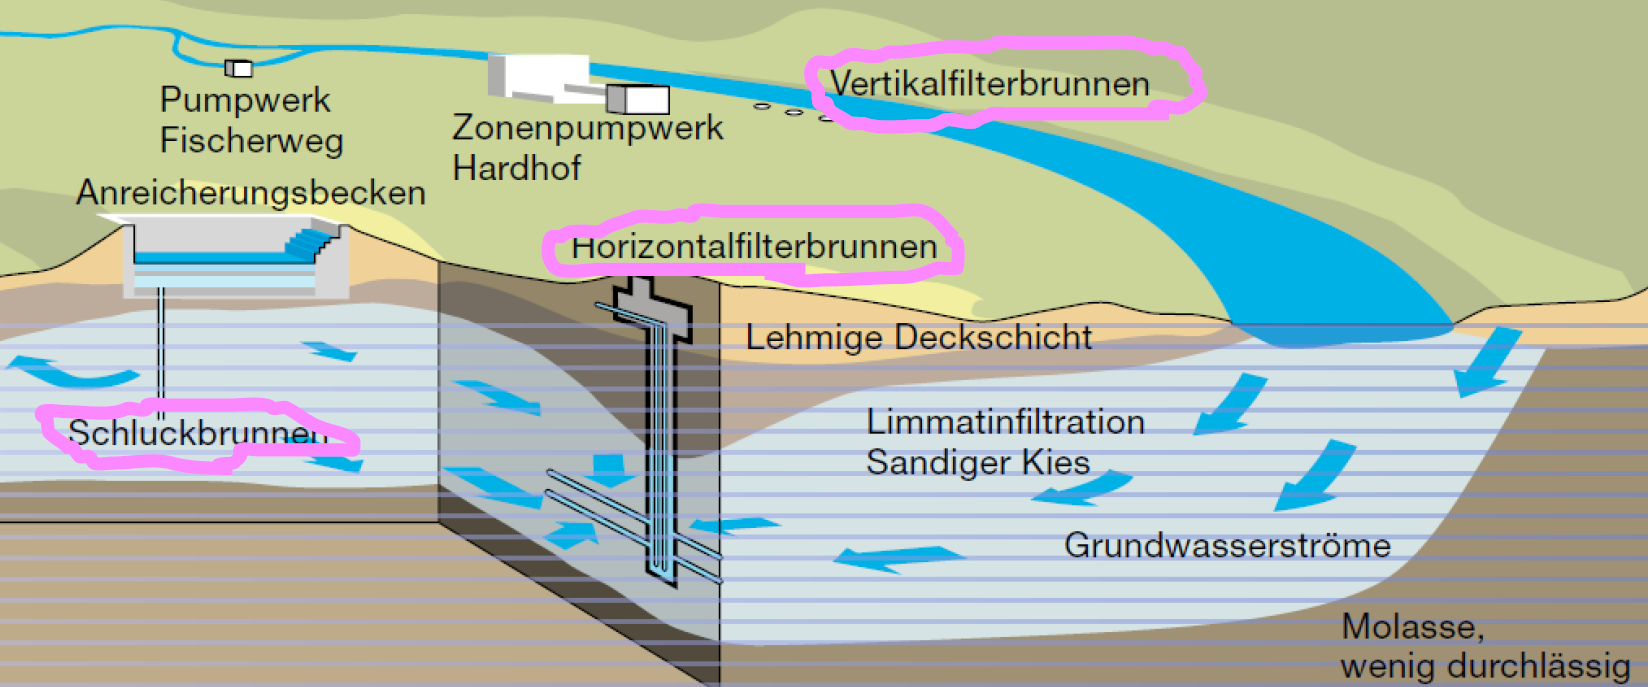
\includegraphics[width=0.9\linewidth]{images/GW2Fassung.PNG} \\
	
	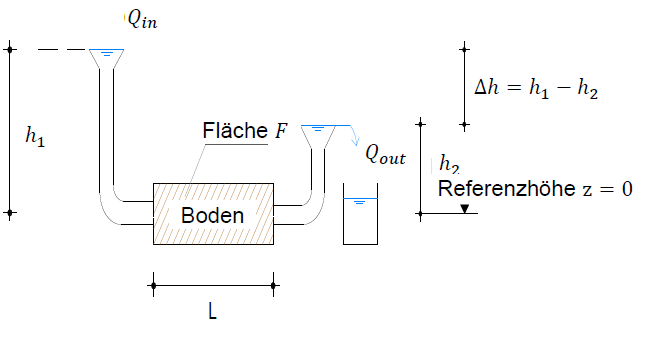
\includegraphics[width=\linewidth]{images/GW3Darcy.PNG} \\
\end{minipage}	
\begin{minipage}{0.7\linewidth}
	\subsection{Gesetz von Darcy}
	\begin{tabular}{p{0.25\linewidth}|l|p{0.4\linewidth}}
		Bemerkung	&	Formel			&	Def \\ \hline
		Bernoulli	&	$ h = z + \frac{u}{\gamma_w} $	&	h: Druckhöhe [m] \\
		Druckhöhe	&					& u: Porenwasserdruck [kPa] \\
					&					& z: Referenzhöhe [m.ü.M] \\ \hline
		Kontinuitätsgleichung	&	$ Q = v \cdot F $ 	& Q: Durchflussmenge [$ \frac{m^3}{s} $] \\
		Grundwasserleiter &					& v: Fliessgeschwindigkeit [ $ \frac{m}{s} $ ] \\ \hline
		Darcy		&  $ v = k \cdot\frac{\Delta h}{L} = k \cdot i $ &	i: hydraulischs Gefälle [-] \\
		Grundwasserleiter &				& k: Durchlässigkeitsbeiwert [ $ \frac{m}{s} $ ] \\
					&					& L: Durchströmte Länger [m] \\
					&					& $ \Delta $ h: Differenz der Druckhöhe [m] \\ \hline
		Wahre Geschwindigkeit eines Wasserteilchens &	$ v_{wahr} = \frac{v}{n} > v $	&	n: Porosität [-] \\
					&					& v: durchschnittliche Geschwindigkeit über ges. Bodenquerschnitt F \\
	\end{tabular}
%\end{minipage}
%\begin{minipage}{\linewidth}
	%	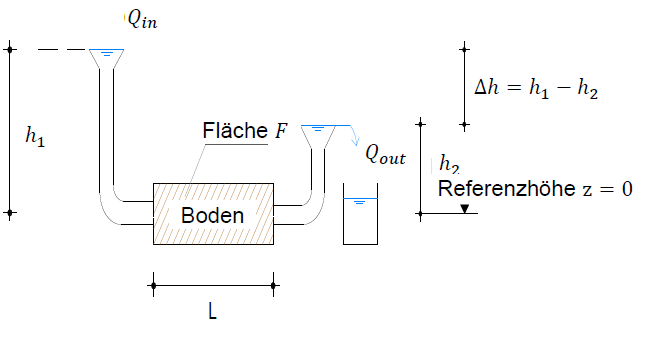
\includegraphics[width=\linewidth]{images/GW3Darcy.PNG} \\
\end{minipage}
\begin{minipage}{0.4\linewidth}
	\subsection{Durchlässigkeit k von Böden}
		
	Entwässerbarkeit:
	\begin{enumerate}
		\item gut wenn: k > 10$^{-3} \frac{cm}{s} $
		\item schlecht 10$^{-4}\frac{cm}{s} \geq k \geq 10^{-6} \frac{cm}{s} $
		\item undurchlässig k < 10$^{-6} \frac{cm}{s} $
	\end{enumerate}
\end{minipage}
\begin{minipage}{0.5\linewidth}
	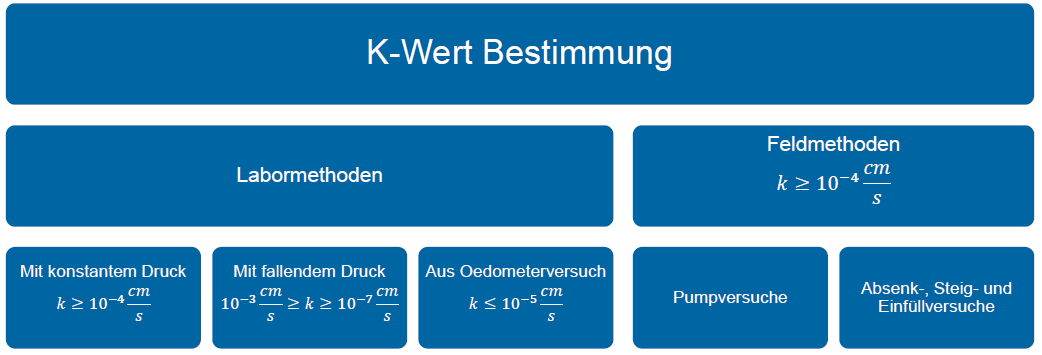
\includegraphics[width=\linewidth]{images/GW4Durchlaessigkeit.PNG} \\
\end{minipage}




\begin{landscape}


\begin{minipage}{0.5\linewidth}
	\subsubsection{Labor}
	
	\begin{tabular}{p{0.25\linewidth}|l|p{0.5\linewidth}}
		Bemerkung	& Formel			&	Def	 \\ \hline
		
		konstante Druckhöhe 	&	$ k = \frac{q \cdot L}{F \cdot \Delta h \cdot t} $	& q: Messvolumen Wasser [$m^3$] \\
		$ \rightarrow $ Sande/Kiese &	& t: Messperiode [s] \\ 
					&					& 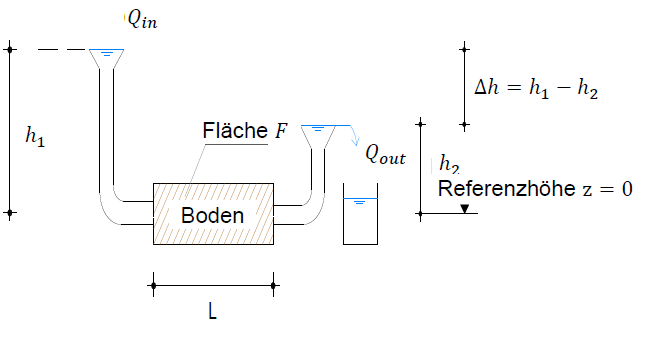
\includegraphics[width=\linewidth]{images/GW3Darcy.PNG} \\ \hline
		
		fallende Druckhöhe $ \rightarrow $ Silte	& $ k = \frac{a \cdot L}{F \cdot (t_2 - t_1) ln \frac{h_1}{h_2}} $	& \\
					&		& \vspace*{-1.25cm} 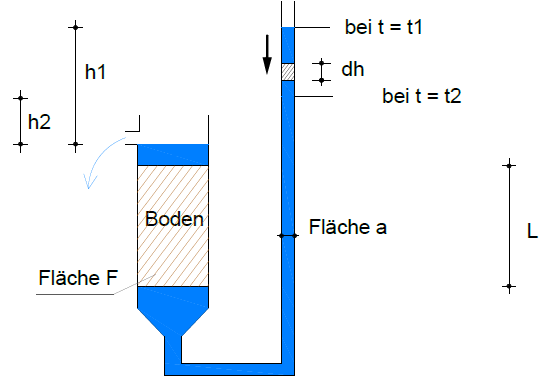
\includegraphics[width=0.8\linewidth]{images/GW5kfall.PNG} \\ \hline
		
		Zeit-Setzungskurve	& $ k = \frac{a_v \cdot \gamma_w \cdot 0.197 \cdot H^2}{(1 + e_m) t_{50}} $ & $a_v$: Verdichtungsbeiwert $ \frac{e_1 - e_2}{\sigma_1 - \sigma_2}$ \\
		$ \rightarrow $ Tone &			& $e_m$ : mittlere Porenziffer \\
					&					& 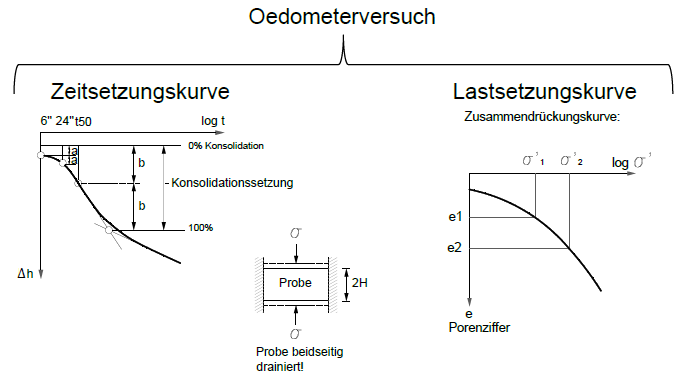
\includegraphics[width=\linewidth]{images/GW6Oedometer.PNG} \\
		
	\end{tabular}
\end{minipage}
\begin{minipage}{\linewidth}
	
	\subsubsection{Feld}
	
	
	\begin{tabular}{l|l|p{0.2\linewidth}}
		Bemerkung	& Formel			&	Def	 \\ \hline
		
		Pumpversuch nach Dupuit & $ k = \frac{Q}{\pi \cdot c} $ & $ c= \frac{H^2 - h_1^2}{ln \frac{R}{r_i} }$  \\
					&					& $ c = \frac{tan( \alpha ) }{2.3} $ \\
					&					& 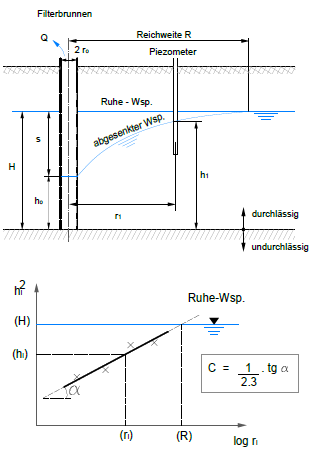
\includegraphics[width=\linewidth]{images/GW7Pump.PNG}  \\ \hline
		
		Pumpversuch nach Sichardt & $ R \widehat{\approx} 3000 \cdot s \sqrt{k} $ & R [m], s [m], k [ $ \frac{m}{s} $ ]  \\ \hline
		
		Absenk-/Steigversuch & $ k = c \frac{1}{h_m} \frac{\Delta h}{\Delta
		 t} $	& \smallskip 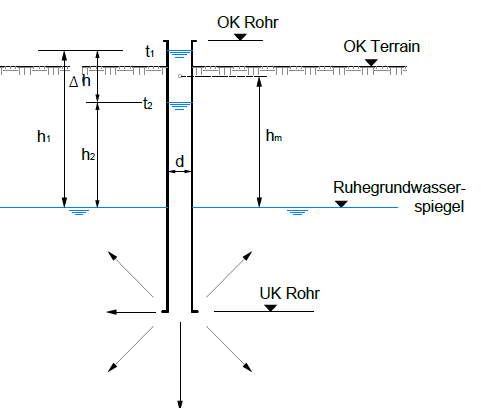
\includegraphics[width=\linewidth]{images/GW8Absenk.PNG}  \\ \hline
		
		Einfüllversuch & $ k = c \frac{1}{h} \frac{4Q}{\pi \cdot d^2} $  &\\
		
	\end{tabular}
\end{minipage}
%\begin{minipage}{\linewidth}
%	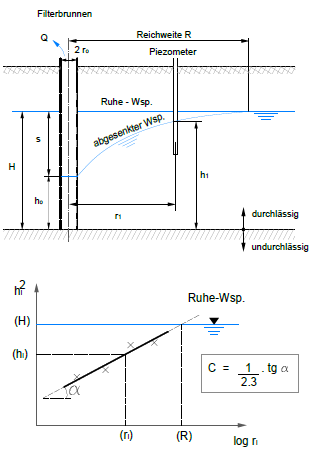
\includegraphics[width=0.35\linewidth]{images/GW7Pump.PNG} \\
%	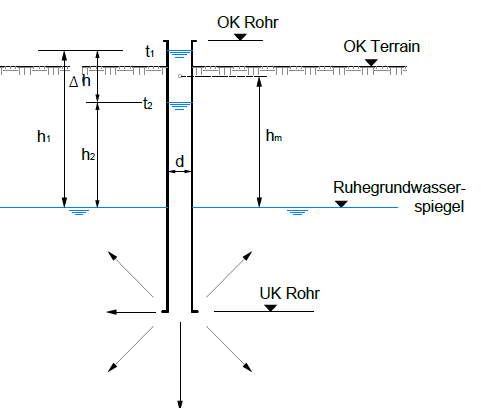
\includegraphics[width=0.35\linewidth]{images/GW8Absenk.PNG} \\
%\end{minipage}

%\end{landscape}



%\begin{minipage}{0.6\linewidth}
%\subsection{Absenkbrunnen}
%	
%	\begin{itemize}
%		\item Offene Wasserhaltung: kleine Bauvorhaben, geringe Absenkung
%		\item Kleine Filterbrunnen: kleinere Bauvorhaben, durchlässige Böden
%		\item Grosse Filterbrunnen: grosse Bauvorhaben, durchlässige Böden
%		\item Wellpoint:kleine bis grosse Bauvorhaben, undurchlässige Böden (min 1.5 m Abstand zwischen Lanzen)
%		
%	\end{itemize}
%
%%\end{minipage}
%%
%%\begin{minipage}{0.5\linewidth}
%		\begin{tabular}{p{0.3\linewidth}|l|p{0.25\linewidth}}
%					
%			\multicolumn{3}{c|}{ \textbf{ungespannter Aquifer} } \\ \hline
%			
%			Vollkommener Vertikalbrunnen (Dupuit-Thiem) & $ Q = \pi \cdot k \frac{H^2 - h_0^2}{ln \frac{R}{r_0} } $	& \smallskip 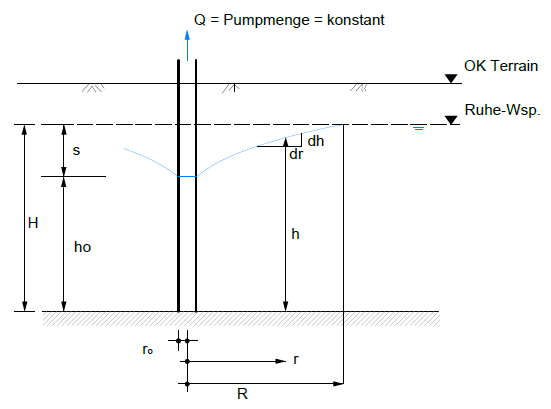
\includegraphics[width=\linewidth]{images/GW9ungespAquifer.PNG}  \\
%			Filterergiebigkeit & $ v_{Grenz} \hat{\approx} \frac{\sqrt{k}}{15}$	& [ $ \frac{m}{s} $ ] \\ \hline
%			
%			\multicolumn{3}{c|}{ \textbf{gespannter Aquifer} } \\ \hline
%			
%			Vollkommener Vertikalbrunnen (Dupuit-Thiem) & $ Q = 2 \cdot \pi \cdot m \cdot k \frac{H - h_0}{ln \frac{R}{r_0} } $	& \smallskip 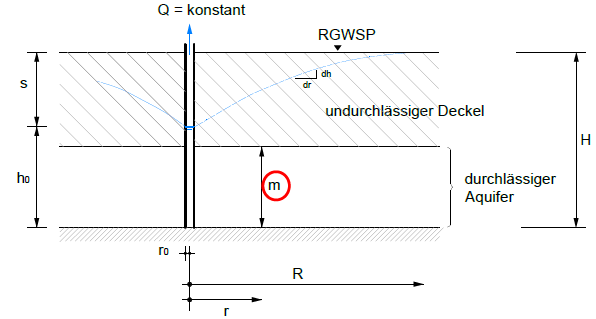
\includegraphics[width=\linewidth]{images/GW10gespAquifer.PNG}  \\ \hline
%			
%			Unvollkommener Vertikalbrunnen (der Brunnen reicht nicht bis zur undurchlässigen Stauschicht)	& $ Q_{unvollk} \approx (1.1 \div 1.3) \cdot Q_{vollk} (H = H_1) $	& \smallskip 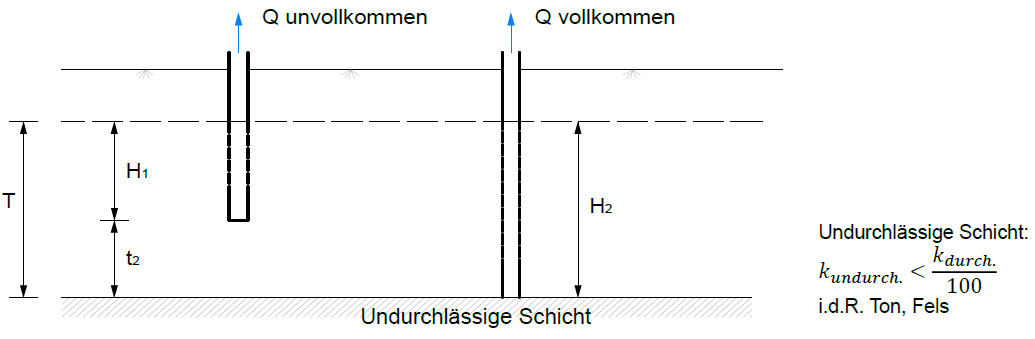
\includegraphics[width=\linewidth]{images/GW11gespAquiferunvollk.PNG}  \\
%						
%		\end{tabular}
%	\end{minipage}
%	\begin{minipage}{0.4\linewidth}
%		
%		\subsubsection{Weitere Grundwasseranwendungen}
%		
%		\begin{tabular}{p{0.3\linewidth}|p{0.35\linewidth}|p{0.3\linewidth}}
%			Bemerkung 		& Formel			&	Einheit \\ \hline
%			
%			Zufluss zu Bach (ungespannt) & $ Q = k \frac{H^2 - L^2}{r \cdot R} $	& \smallskip 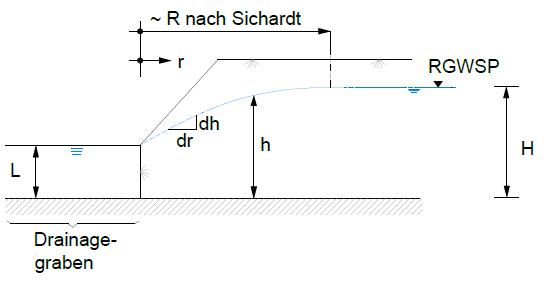
\includegraphics[width=\linewidth]{images/GW12Bachungespannt.PNG}  \\ \hline
%			
%			Zufluss zu Bach (gespannt)	& $ Q = m \cdot k \frac{H - L}{R} $ & \smallskip 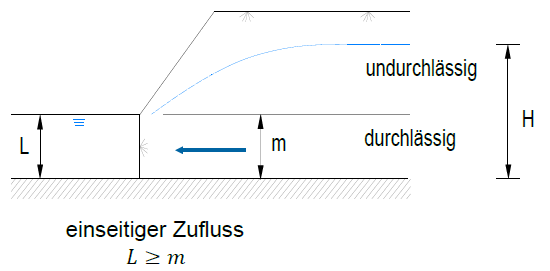
\includegraphics[width=\linewidth]{images/GW13Bachgespannt.PNG}  \\ \hline
%			
%			GW-Absenkung für Baugrube mit mehreren Brunnen 	& 1. Fiktiver Radius R$_A = \sqrt{\frac{a \cdot b}{\pi} } $ [m]	& R$_A$ : fiktiver Radius (Baugrubenabmessung a x b) $ R_A = \sqrt{ \frac{a \cdot b }{\pi} } $ \\
%															& 2. Abschätzung Pumpwassermenge Q$_{tot} =\pi \cdot k \frac{H^2 - h^2}{ln(R) - ln(R_A) } $ [$ \frac{m^3}{s} $]												& \smallskip \multirow{7}{*}{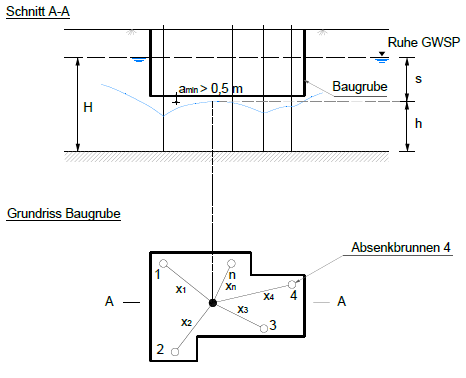
\includegraphics[width=\linewidth]{images/GW14mehrereBrunnen.PNG} }  \\
%															& 3. v$_{Grenz} = \frac{ \sqrt{k} }{15} $ [$ \frac{m}{s} $]		& \\
%															& 4. erf. benetzte Brunnenmantelfläche $ M_{erf} = \frac{Q_{tot} }{v_{Grenz} } [m^2]$ & \\
%															& 5. Filterhöhe $ h = \frac{M_{erf} }{U_{Brunnen} } $ [m] $ \rightarrow $ Faktor 2 Sicherheit bei Anzahl Brunnen												& \\
%															& 6. GW-Spiegelhöhe z an beliebiger Stelle $ z = \sqrt{ H^2 - \frac{Q_{tot} }{\pi \cdot k} [ln(R) - \frac{1}{n} ln(x_i) ] } $								& \\
%															& 7. Pumpwassermenge an beliebiger Stelle Q$_{f} = \pi \cdot k \frac{H^2 - z^2 }{ln(R) - \frac{1}{n} ln(x_1 \cdot x_2 \cdot ... x_n) } $					& \\
%															& 8. Pumpwassermenge pro Brunnen Q$_{erf} = \frac{Q_f}{n} $		& \\
%%			\begin{enumerate}
%%				\item Fiktiver Radius R$_A = \sqrt{\frac{a \cdot b}{\pi} } $ [m]
%%				\item Abschätzung Pumpwassermenge Q$_{tot} =\pi \cdot k \frac{H^2 - h^2}{ln(R) - ln(R_A) } $ [$ \frac{m^3}{s} $]
%%				\item v$_{Grenz} = \frac{ \sqrt{k} }{15} $ [$ \frac{m}{s} $]
%%				\item erf. benetzte Brunnenmantelfläche $ M_{erf} = \frac{Q_{tot} }{v_{Grenz} } [m^2]$
%%				\item Filterhöhe $ h = \frac{M_{erf} }{U_{Brunnen} } $ [m] $ \rightarrow $ Faktor 2 Sicherheit bei Anzahl Brunnen
%%				\item GW-Spiegelhöhe z an beliebiger Stelle $ z = \sqrt{ H^2 - \frac{Q_{tot} }{\pi \cdot k} [ln(R) - \frac{1}{n} ln(x_i) ] } $
%%				\item Pumpwassermenge an beliebiger Stelle Q$_{f} = \pi \cdot k \frac{H^2 - z^2 }{ln(R) - \frac{1}{n} ln(x_1 \cdot x_2 \cdot ... x_n) } $
%%				\item Pumpwassermenge pro Brunnen Q$_{erf} = \frac{Q_f}{n} $
%%			\end{enumerate}
%%		& R$_A$ : fiktiver Radius (Baugrubenabmessung a x b) $ R_A = \sqrt{ \frac{a \cdot b }{\pi} } $ \\
%%							&					& \smallskip 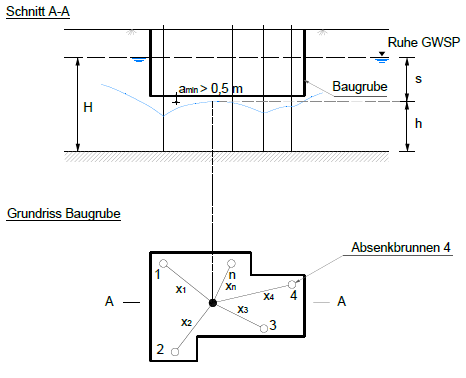
\includegraphics[width=\linewidth]{images/GW14mehrereBrunnen.PNG}  \\ \hline
%			
%		\end{tabular}
%	\end{minipage}

\end{landscape}

\begin{minipage}{\linewidth}
	\vspace{-0.5cm}
	\subsection{Absenkbrunnen}
	
	\begin{itemize}
		\item Offene Wasserhaltung: kleine Bauvorhaben, geringe Absenkung
		\item Kleine Filterbrunnen: kleinere Bauvorhaben, durchlässige Böden
		\item Grosse Filterbrunnen: grosse Bauvorhaben, durchlässige Böden
		\item Wellpoint:kleine bis grosse Bauvorhaben, undurchlässige Böden (min 1.5 m Abstand zwischen Lanzen)
		
	\end{itemize}
	
	%\end{minipage}
	%
	%\begin{minipage}{0.5\linewidth}
	\begin{tabular}{p{0.3\linewidth}|l|p{0.25\linewidth}}
		
		\multicolumn{3}{c|}{ \textbf{ungespannter Aquifer} } \\ \hline
		
		Vollkommener Vertikalbrunnen (Dupuit-Thiem) & $ Q = \pi \cdot k \frac{H^2 - h_0^2}{ln \frac{R}{r_0} } $	& \multirow{2}{*}{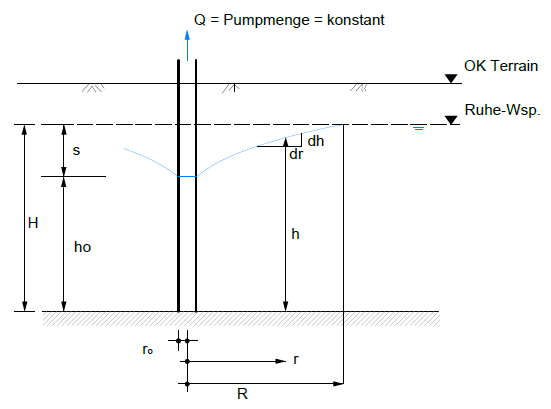
\includegraphics[width=0.8\linewidth]{images/GW9ungespAquifer.PNG}}  \\
		Filterergiebigkeit & $ v_{Grenz} \hat{\approx} \frac{\sqrt{k}}{15}$	&\\ \hline
		
		\multicolumn{3}{c|}{ \textbf{gespannter Aquifer} } \\ \hline
		
		Vollkommener Vertikalbrunnen (Dupuit-Thiem) & $ Q = 2 \cdot \pi \cdot m \cdot k \frac{H - h_0}{ln \frac{R}{r_0} } $	& \smallskip 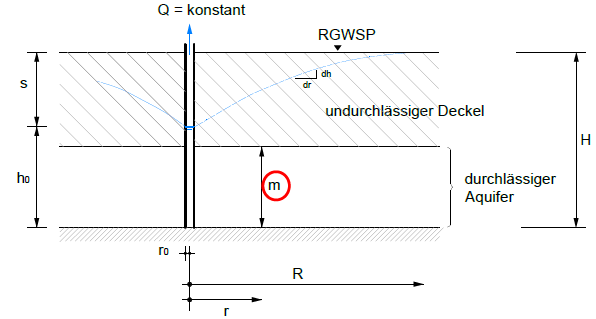
\includegraphics[width=0.8\linewidth]{images/GW10gespAquifer.PNG}  \\ \hline
		
		Unvollkommener Vertikalbrunnen (der Brunnen reicht nicht bis zur undurchlässigen Stauschicht)	& $ Q_{unvollk} \approx (1.1 \div 1.3) \cdot Q_{vollk} (H = H_1) $	& \smallskip 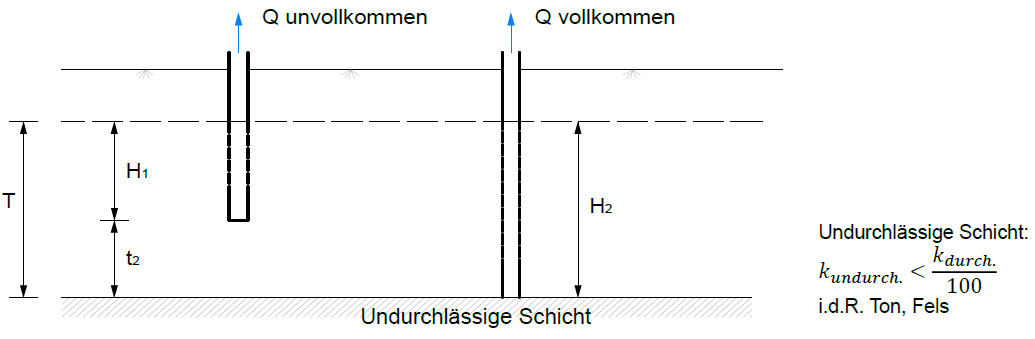
\includegraphics[width=\linewidth]{images/GW11gespAquiferunvollk.PNG}  \\
		
	\end{tabular}
\end{minipage}
\begin{minipage}{\linewidth}
	
	\subsubsection{Weitere Grundwasseranwendungen}
	
	\begin{tabular}{p{0.2\linewidth}|p{0.5\linewidth}|p{0.25\linewidth}}
		Bemerkung 		& Formel			&	Einheit \\ \hline
		
		Zufluss zu Bach (ungespannt) & $ Q = k \frac{H^2 - L^2}{r \cdot R} $	& \smallskip 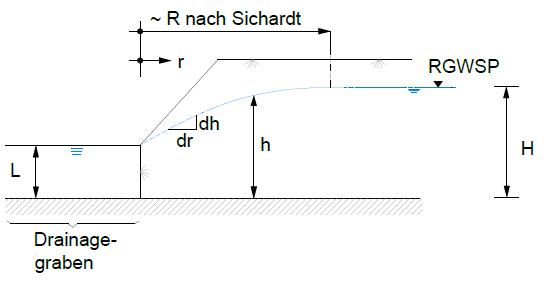
\includegraphics[width=\linewidth]{images/GW12Bachungespannt.PNG}  \\ \hline
		
		Zufluss zu Bach (gespannt)	& $ Q = m \cdot k \frac{H - L}{R} $ & \smallskip 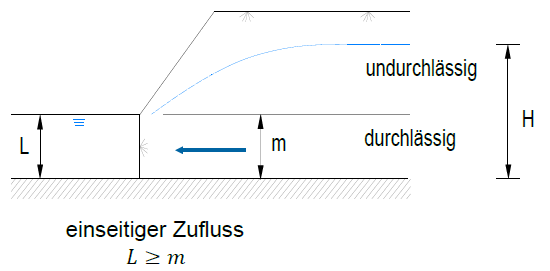
\includegraphics[width=\linewidth]{images/GW13Bachgespannt.PNG}  \\ \hline
		
		GW-Absenkung für Baugrube mit mehreren Brunnen 	& 1. Fiktiver Radius R$_A = \sqrt{\frac{a \cdot b}{\pi} } $ [m]	& R$_A$ : fiktiver Radius (Baugrubenabmessung a x b) $ R_A = \sqrt{ \frac{a \cdot b }{\pi} } $ \\
		& 2. Abschätzung Pumpwassermenge Q$_{tot} =\pi \cdot k \frac{H^2 - h^2}{ln(R) - ln(R_A) } $ [$ \frac{m^3}{s} $]												& R = 3000 $\cdot$ s $\cdot$ $\sqrt{k}$ \smallskip \multirow{7}{*}{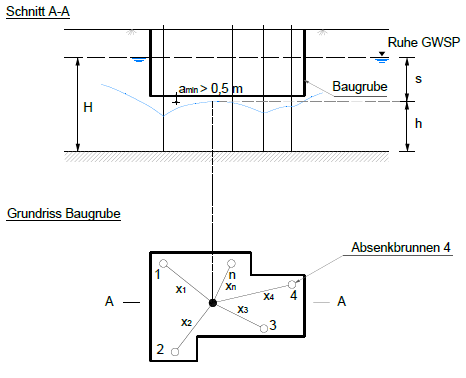
\includegraphics[width=\linewidth]{images/GW14mehrereBrunnen.PNG} }  \\
		& 3. v$_{Grenz} = \frac{ \sqrt{k} }{15} $ [$ \frac{m}{s} $]		& \\
		& 4. erf. benetzte Brunnenmantelfläche $ M_{erf} = \frac{Q_{tot} }{v_{Grenz} } [m^2]$ & \\
		& 5. Filterhöhe $ h = \frac{M_{erf} }{U_{Brunnen} } $ [m] $ \rightarrow $ Faktor 2 Sicherheit bei Anzahl Brunnen												& \\
		& 5.1 Anzahl Brunnen $ n = \frac{Q_{tot}}{v_{Grenz} \cdot U_B \cdot h} $	& \\
		& 6. GW-Spiegelhöhe z an beliebiger Stelle $ z = \sqrt{ H^2 - \frac{Q_{tot} }{\pi \cdot k} [ln(R) - \frac{1}{n} ln(x_i) ] } $								& \\
		& 7. Pumpwassermenge an beliebiger Stelle Q$_{f} = \pi \cdot k \frac{H^2 - z^2 }{ln(R) - \frac{1}{n} ln(x_1 \cdot x_2 \cdot ... x_n) } $					& \\
		& 8. Pumpwassermenge pro Brunnen Q$_{erf} = \frac{Q_f}{n} $		& Sandfreiheit v < 2.9 $\cdot 10^{-3} $  \\
		
	\end{tabular}
\end{minipage}

%\clearpage

	\begin{minipage}{\linewidth}
		
		\subsubsection{Sickernetze}
		
		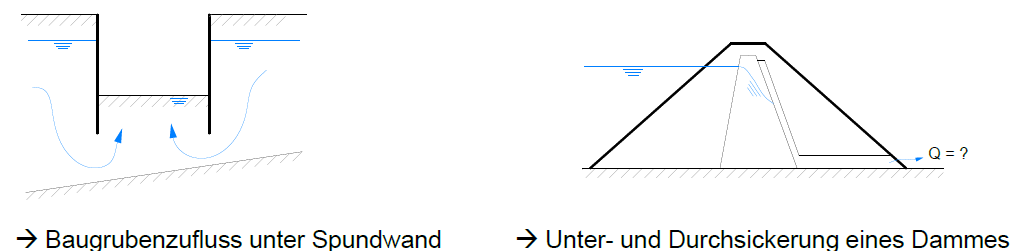
\includegraphics[width=0.6\linewidth]{images/GW15Sickerwassermenge.PNG}
		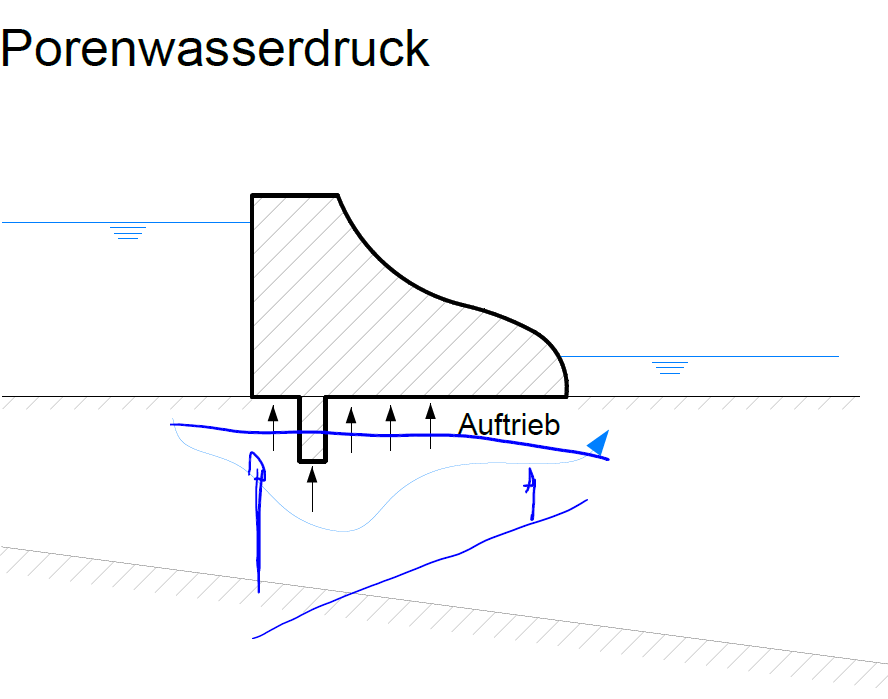
\includegraphics[width=0.2\linewidth]{images/GW16Porenwasserdruck.PNG}		\\
	\end{minipage}
\begin{minipage}{0.5\linewidth}
		
		\textbf{Konstruktion von Sickernetzen}
		\begin{enumerate}
			\item QS aufzeichnen (Massstab, mögl. quadratisch)
			\item Begrenzung einzeichnen (undurchlässige Schichten, Bäche, Seen)
			\item Sickernetz konstruieren (Potentiallinien, Stromlinien)
					$ \rightarrow $ N$_f$ = Anzahl Stromröhren (in jeder Stromröhre fliesst gleichviel GW); N$_d$ = Anzahl Potentialstufen (auf einer Potentiallinie ist gleicher Wasserdruck/gl. Piezometerhöhe)
			\item Formeln:			
		\end{enumerate}
		\begin{itemize}
			\item Durchfluss pro Rohr: $ \Delta Q = k \cdot \frac{\Delta H}{\Delta L} \cdot \Delta b $
			\item $ v = k \cdot i $
			\item $ i = \frac{\Delta H}{\Delta L} $
			\item $ Q = N_f \cdot \Delta Q $
			\item $ H = N_d \cdot \Delta H $
			\item $ Q = k \cdot H \cdot \frac{N_f}{N_d} $ [ $ \frac{m^3}{s \cdot m^l} $ ]
			\item Wasserdruck/Piezometer: $ h = H - \frac{H}{N_d} \cdot n $ [m] $ \rightarrow \cdot 10 = u [\frac{kN}{m^2}] $; wobei n = Anzahl Felder
			\item Auftrieb: $ A = u \cdot L \cdot B $ [kN]
		\end{itemize}
	
\end{minipage}
\begin{minipage}{0.4\linewidth}
	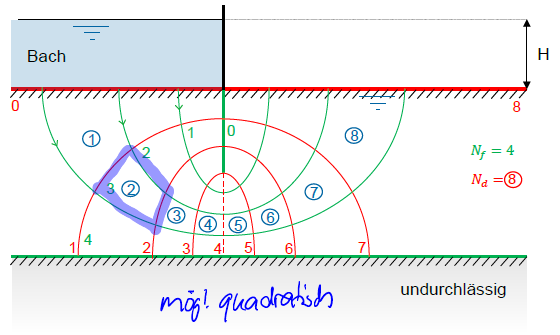
\includegraphics[width=\linewidth]{images/GW17Sickernetz.PNG}
\end{minipage}





\begin{minipage}{0.7\linewidth}
	
	\subsubsection{Hydraulischer Grundbruch}
	
	\begin{tabular}{p{0.23\linewidth}|l|l}
				
		\multicolumn{3}{c}{\textbf{Strömungsdruck} } \\ \hline
		
		Strömungsgradient &	$ i_{vorh} = \frac{\Delta H}{t} $	& $\Delta$ H: Absenkung GW [m] \\
					&					& t: Einbindetiefe [m] \\
					&	$ i_{krit} = \frac{\gamma'}{\gamma_w} $	& \\
		Sicherheit  &	$ F = \frac{i_{krit} }{i_{vorh} } $	& auflösen nach t [m] \\ \hline
		
		Einbindetiefe anisotropisches Zuströmen neues Konzept nach SIA 267 &	$ \gamma' \cdot \gamma_{G,inf} \geq \gamma_w \cdot i_{vorh} \cdot \gamma_{G,sup} $	& $\gamma_{G}$: Sia 260, Tab. 1	\\
		
		Porenwasserdruck & $ u = u_0 - \Delta u = u_0 - i \cdot \gamma_w \cdot z $ & \\
		
		Effektive Spannung & $ \sigma_v' = \sigma_v - u = \sigma_{v,0}' + \Delta u $	& \\
		
		Gewicht Bodenelement unter Auftrieb & $ G = \gamma' \cdot V $	& \\
		
		Strömungskraft	& $ S = \gamma_w \cdot i \cdot V $	& \\
		
		Resultierende Auf-/Abwärtsströmung & $ R = (\gamma' \pm \gamma_w \cdot i) \cdot V $	& \\ \hline
		
		Sicherheit	& $ F = \frac{G}{S} $	& \\
		
		
		\multicolumn{3}{c}{\textbf{Wasserdrücke im Boden} } \\ \hline
		
		hydrostatischer Druck	& $ w = \gamma_w \cdot t $	&	\\
		
		mit Aufwärtsströmung	& $ w = \gamma_w (1 + i) t $	& \\
		
		mit Abwärtsströmung		& $ w = \gamma_w (1 - i) t $	& \\
		
		seitliche Kraft aus Wasserdruck & $ W = 0.5 \cdot t \cdot w = 0.5 \cdot t^2 \cdot \gamma_w $	& [ $ \frac{kN}{m^l} $ ] \\
		
		Auftriebkraft	& $ A = w \cdot b = t \cdot b \cdot \gamma_w $ & [ $ \frac{kN}{m^l} $ ] \\
		
		Bemesseung		& $ G \geq F_s \cdot A $	& F$_s = \frac{\gamma_{G,sup}}{\gamma_{G,inf}} \geq 1.1 \div 1.2 $ \\
		
		
	\end{tabular}
\end{minipage}
\begin{minipage}{0.3\linewidth}
	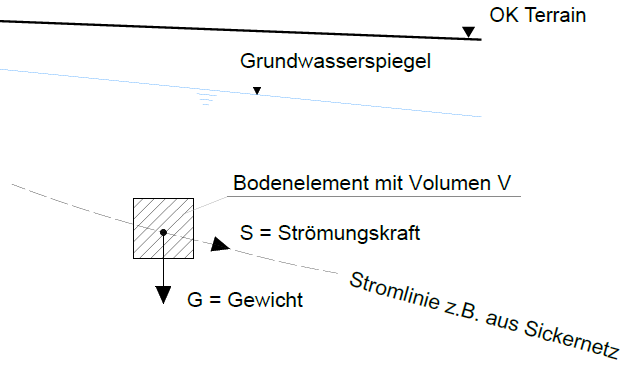
\includegraphics[width=\linewidth]{images/GW18Kraftwirkung.PNG}
	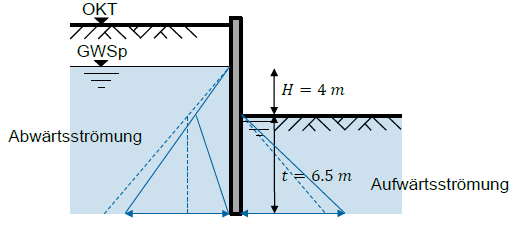
\includegraphics[width=\linewidth]{images/GW19Stroemungsdruck.PNG}
%	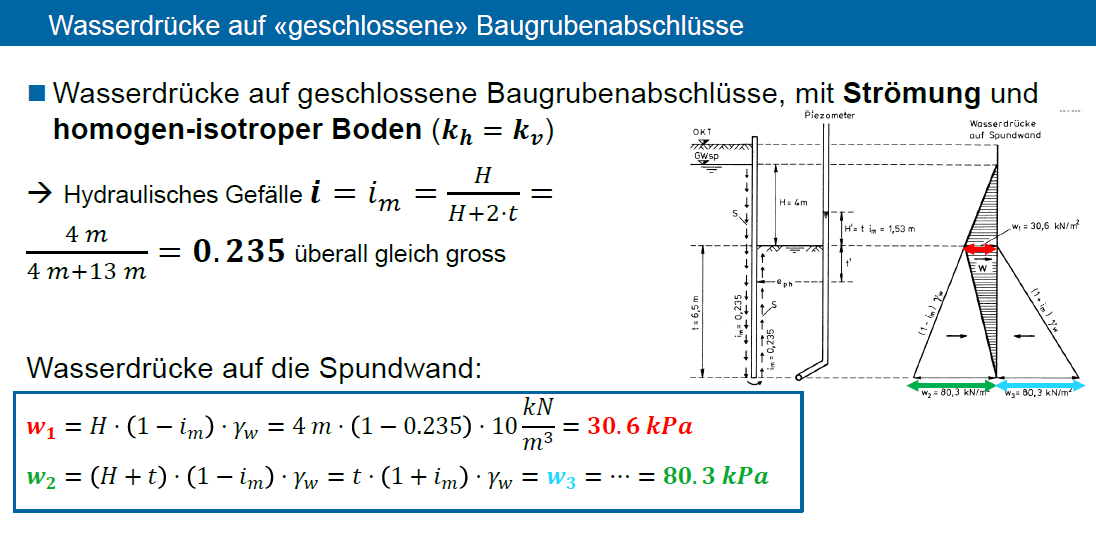
\includegraphics[width=\linewidth]{images/GW20Wasserdrucke.PNG}
	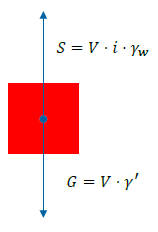
\includegraphics[width=0.5\linewidth]{images/GW21Kraftwirkung.PNG}
\end{minipage}
	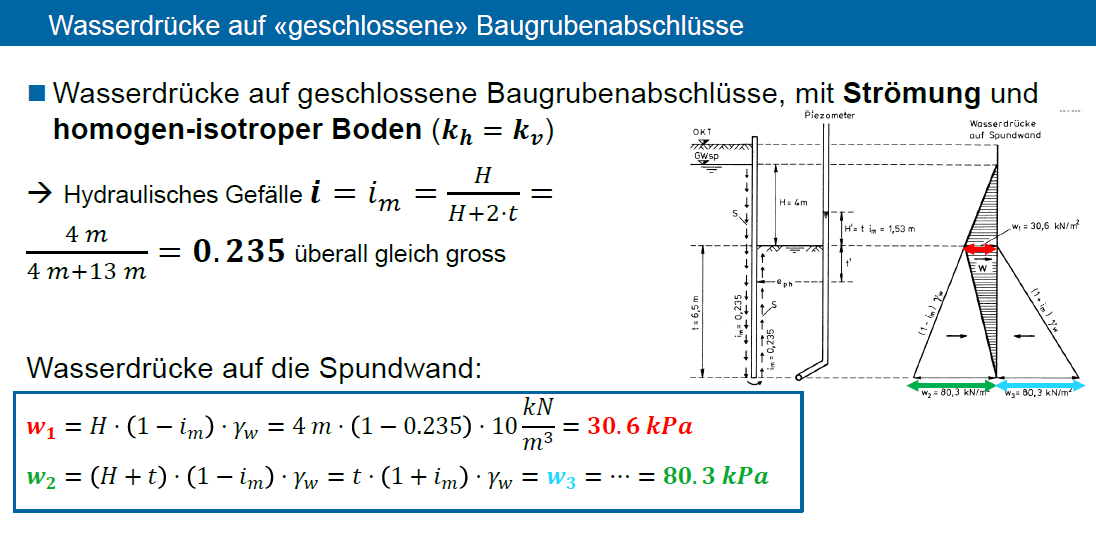
\includegraphics[width=0.9\linewidth]{images/GW20Wasserdrucke.PNG}
\clearpage
\section{Böschungsstabilität}

Rutschbewegungen: gerade oder Kreisförmig \\
Strömendes Wasser verringert, stehendes Wasser erhöht Sicherheitsgrad
\subsection{Kinematische Methode}
\subsubsection{Methode Culmann}
$ \beta > \varphi_m $ sonst kein Versagen \\
$ F < 1 $ Versagen \\
\\
\begin{minipage}{0.55\linewidth}
		\textbf{Vorgehen}:
		\begin{enumerate}
			\item $ F_{\varphi_0} = \textcolor{red}{1} $
			\item mobilisierte Reibungswinkel $ \varphi_m = arctan \frac{tan (\varphi_0)}{\textcolor{red}{F_{\varphi_0}}} $
			\item $ N_s = \frac{4 sin (\beta) cos \textcolor{red}{(\varphi_m)}}{1 - cos (\beta - \textcolor{red}{\varphi_m})} $
			\item $ c_m = \frac{\gamma \cdot H}{\textcolor{red}{N_s}} $
			\item $ F_{c0} = \frac{c}{\textcolor{red}{c_m}} $
			\item Überprüfen: $ F_{c0} = \textcolor{red}{F_{\varphi_0}} \rightarrow $ wenn ja: i.O, wenn nein: Iteration
		\end{enumerate}
\end{minipage}
\begin{minipage}{0.5\linewidth}
	\textbf{Bodenparameter} \\
	\begin{tabular}{l|l|l|l}
					&	Drainiert			& Undrainiert			& Einheit \\ \hline
		
	Bodengewicht	&	$ \gamma' $			& $ \gamma = \gamma_g $ & $ [\frac{kN}{m^3}] $ \\
	Reibungswinkel	&	$ \varphi' $		& $ \varphi  $			& [°] \\
	Kohäsion		& c'					&  s$_u $				& $[ \frac{kN}{m^2} ]$ \\
	Sicherheitsfaktor & $ F=\frac{c}{c_m} $	& $ F=\frac{s_u}{s_m} $	& \\
	
	\end{tabular}
\end{minipage}


\subsubsection{Methode Taylor}
\textcolor{red}{Farbiges Diagramm} \\
	\begin{minipage}{\linewidth}
		genauer als Culmann bei steiler Böschung (Taylor arbeitet mit Bruchkreisen), Berechnung gem. Culmann ausser Schritt 3
		
		\hspace{0.5cm} 3. $ N_s $ aus Diagramm $ \rightarrow \frac{1}{N_s} $
	\end{minipage}

\subsubsection{Methode Michalowski}
	\begin{minipage}{\linewidth}
		Basiert auf unterschiedlicher Bruchform als Taylor \\
	\end{minipage}





\subsection{Lamellen Methode}

	\begin{minipage}{0.25\linewidth}
		\includegraphics[width=\linewidth]{images/Boschstab1Lamelle.jpg} \\
% \end{minipage}
% \begin{minipage}{\linewidth}
		\includegraphics[width=\linewidth]{images/Boschstab2Krafte.PNG} \\
	\end{minipage}
\begin{minipage}{\linewidth}
	
	\begin{align*}		
		G' 	&= ( \gamma \cdot z_d + \gamma' \cdot z_s ) \Delta x  \\
		S_w	&= \gamma_w \cdot \Delta x \cdot sin(\beta) \cdot z_s \\
		M_E	&= G' \cdot sin(\alpha) + S_w \cdot cos(\alpha - \beta) \cdot R \\
		M_R	&= [G' \cdot sin(\alpha) - S_w \cdot sin(\alpha - \beta) ] \cdot tan(\varphi')R + c' \frac{\Delta x}{cos(\alpha)} R
	\end{align*}

\end{minipage}
\begin{minipage}{\linewidth}
	
	\begin{tabular}{l|l|l|l|l|l|l|l|l|l|l|l|l|l|l}
				& $ \Delta $ x	& (x)	& $ \alpha $	& $ \beta $	& c'	& $ \varphi' $	& $ \gamma $	& $ \gamma' $	& z$_d$	& z$_s$	& G'	& S$_w$	&	M$_E$	& M$_R$	\\ \hline
			
			Nr	& m	& m	& °	& °	& kPa	& °	& $ \frac{kN}{m^3} $	& $ \frac{kN}{m^3} $	& m	& m	& $ \frac{kN}{m} $	& $ \frac{kN}{m} $	& $ \frac{kN}{m} $	& $ \frac{kN}{m} $ \\ \hline
			
			1 &&&&&&&&&&&&&& \\
			2 &&&&&&&&&&&&&& \\
			3 &&&&&&&&&&&&&& \\
			... &&&&&&&&&&&&&& \\ \hline
			&&&&&&&&&&&&& $  \sum M_E $ & $  \sum M_R $ \\
			&&&&&&&&&&&&& \multicolumn{2}{c|}{$ F = \frac{M_R}{M_E}$} \\
	\end{tabular}

\end{minipage}
\clearpage

%\begin{minipage}{\linewidth}
	\vspace{-0.5cm}
\subsection{Absenkbrunnen}
	
	\begin{itemize}
		\item Offene Wasserhaltung: kleine Bauvorhaben, geringe Absenkung
		\item Kleine Filterbrunnen: kleinere Bauvorhaben, durchlässige Böden
		\item Grosse Filterbrunnen: grosse Bauvorhaben, durchlässige Böden
		\item Wellpoint:kleine bis grosse Bauvorhaben, undurchlässige Böden (min 1.5 m Abstand zwischen Lanzen)
		
	\end{itemize}

%\end{minipage}
%
%\begin{minipage}{0.5\linewidth}
		\begin{tabular}{p{0.3\linewidth}|l|p{0.25\linewidth}}
					
			\multicolumn{3}{c|}{ \textbf{ungespannter Aquifer} } \\ \hline
			
			Vollkommener Vertikalbrunnen (Dupuit-Thiem) & $ Q = \pi \cdot k \frac{H^2 - h_0^2}{ln \frac{R}{r_0} } $	& \multirow{2}{*}{\includegraphics[width=0.8\linewidth]{images/GW9ungespAquifer.PNG}}  \\
			Filterergiebigkeit & $ v_{Grenz} \hat{\approx} \frac{\sqrt{k}}{15}$	&\\ \hline
			
			\multicolumn{3}{c|}{ \textbf{gespannter Aquifer} } \\ \hline
			
			Vollkommener Vertikalbrunnen (Dupuit-Thiem) & $ Q = 2 \cdot \pi \cdot m \cdot k \frac{H - h_0}{ln \frac{R}{r_0} } $	& \smallskip \includegraphics[width=0.8\linewidth]{images/GW10gespAquifer.PNG}  \\ \hline
			
			Unvollkommener Vertikalbrunnen (der Brunnen reicht nicht bis zur undurchlässigen Stauschicht)	& $ Q_{unvollk} \approx (1.1 \div 1.3) \cdot Q_{vollk} (H = H_1) $	& \smallskip \includegraphics[width=\linewidth]{images/GW11gespAquiferunvollk.PNG}  \\
						
		\end{tabular}
	\end{minipage}
	\begin{minipage}{\linewidth}
		
		\subsubsection{Weitere Grundwasseranwendungen}
		
		\begin{tabular}{p{0.2\linewidth}|p{0.4\linewidth}|p{0.3\linewidth}}
			Bemerkung 		& Formel			&	Einheit \\ \hline
			
			Zufluss zu Bach (ungespannt) & $ Q = k \frac{H^2 - L^2}{r \cdot R} $	& \smallskip \includegraphics[width=\linewidth]{images/GW12Bachungespannt.PNG}  \\ \hline
			
			Zufluss zu Bach (gespannt)	& $ Q = m \cdot k \frac{H - L}{R} $ & \smallskip \includegraphics[width=\linewidth]{images/GW13Bachgespannt.PNG}  \\ \hline
			
			GW-Absenkung für Baugrube mit mehreren Brunnen 	& 1. Fiktiver Radius R$_A = \sqrt{\frac{a \cdot b}{\pi} } $ [m]	& R$_A$ : fiktiver Radius (Baugrubenabmessung a x b) $ R_A = \sqrt{ \frac{a \cdot b }{\pi} } $ \\
															& 2. Abschätzung Pumpwassermenge Q$_{tot} =\pi \cdot k \frac{H^2 - h^2}{ln(R) - ln(R_A) } $ [$ \frac{m^3}{s} $]												& \smallskip \multirow{7}{*}{\includegraphics[width=\linewidth]{images/GW14mehrereBrunnen.PNG} }  \\
															& 3. v$_{Grenz} = \frac{ \sqrt{k} }{15} $ [$ \frac{m}{s} $]		& \\
															& 4. erf. benetzte Brunnenmantelfläche $ M_{erf} = \frac{Q_{tot} }{v_{Grenz} } [m^2]$ & \\
															& 5. Filterhöhe $ h = \frac{M_{erf} }{U_{Brunnen} } $ [m] $ \rightarrow $ Faktor 2 Sicherheit bei Anzahl Brunnen												& \\
															& 6. GW-Spiegelhöhe z an beliebiger Stelle $ z = \sqrt{ H^2 - \frac{Q_{tot} }{\pi \cdot k} [ln(R) - \frac{1}{n} ln(x_i) ] } $								& \\
															& 7. Pumpwassermenge an beliebiger Stelle Q$_{f} = \pi \cdot k \frac{H^2 - z^2 }{ln(R) - \frac{1}{n} ln(x_1 \cdot x_2 \cdot ... x_n) } $					& \\
															& 8. Pumpwassermenge pro Brunnen Q$_{erf} = \frac{Q_f}{n} $		& \\
%			\begin{enumerate}
%				\item Fiktiver Radius R$_A = \sqrt{\frac{a \cdot b}{\pi} } $ [m]
%				\item Abschätzung Pumpwassermenge Q$_{tot} =\pi \cdot k \frac{H^2 - h^2}{ln(R) - ln(R_A) } $ [$ \frac{m^3}{s} $]
%				\item v$_{Grenz} = \frac{ \sqrt{k} }{15} $ [$ \frac{m}{s} $]
%				\item erf. benetzte Brunnenmantelfläche $ M_{erf} = \frac{Q_{tot} }{v_{Grenz} } [m^2]$
%				\item Filterhöhe $ h = \frac{M_{erf} }{U_{Brunnen} } $ [m] $ \rightarrow $ Faktor 2 Sicherheit bei Anzahl Brunnen
%				\item GW-Spiegelhöhe z an beliebiger Stelle $ z = \sqrt{ H^2 - \frac{Q_{tot} }{\pi \cdot k} [ln(R) - \frac{1}{n} ln(x_i) ] } $
%				\item Pumpwassermenge an beliebiger Stelle Q$_{f} = \pi \cdot k \frac{H^2 - z^2 }{ln(R) - \frac{1}{n} ln(x_1 \cdot x_2 \cdot ... x_n) } $
%				\item Pumpwassermenge pro Brunnen Q$_{erf} = \frac{Q_f}{n} $
%			\end{enumerate}
%		& R$_A$ : fiktiver Radius (Baugrubenabmessung a x b) $ R_A = \sqrt{ \frac{a \cdot b }{\pi} } $ \\
%							&					& \smallskip \includegraphics[width=\linewidth]{images/GW14mehrereBrunnen.PNG}  \\ \hline
			
		\end{tabular}
	\end{minipage}
%\clearpage
\end{document}
